%!TEX root = ../larxxia.tex

\section{The inverse of a matrix}
\label{sec:im}

\secttoc

\begin{comment}
\pooliv{p.163--9}  \layiv{\S2.2--3}  \cite[\S3.2]{Nakos1998}  \cite[Ch.~6]{Chartier2015}
\end{comment}


The previous \autoref{sec:moaa} introduced addition, subtraction, multiplication, and other operations of matrices.  
Conspicuously missing from the list is `division' by a matrix.
This section develops `division' by a matrix as multiplication by the inverse of a matrix.
The analogue in ordinary arithmetic is that division by ten is the same as multiplying by its reciprocal, one-tenth.
But the inverse of a matrix looks nothing like a reciprocal.


\subsection{Introducing the unique inverse}

Let's start with an example that illustrates an analogy with the reciprocal\slash inverse of a scalar number.

\begin{example} \label{eg:a2x2inv}
%while abs(det(A))~=1, A=round(randn(2,2)*5), end, B=inv(A)
Recall that a crucial property is that a number multiplied by its reciprocal\slash inverse is one: for example, \(2\times 0.5=1\) so \(0.5\) is the reciprocal\slash inverse of~\(2\).
Similarly, show that matrix 
\begin{equation*}
B=\begin{bmatrix} -3&1\\-4&1 \end{bmatrix}
\text{ is an inverse of }
A=\begin{bmatrix} 1&-1\\4&-3 \end{bmatrix}
\end{equation*}
by showing their product is the \(2\times2\) \idx{identity matrix}~\(I_2\).
\begin{solution} 
Multiply 
\begin{equation*}
AB=\begin{bmatrix} 1&-1\\4&-3 \end{bmatrix}
\begin{bmatrix} -3&1\\-4&1 \end{bmatrix}
=\begin{bmatrix} 1&0\\0&1 \end{bmatrix}=I_2
\end{equation*}
the multiplicative identity.  
But matrix multiplication is generally not commutative (\autoref{sec:fapmo}), so also consider
\begin{equation*}
BA=\begin{bmatrix} -3&1\\-4&1 \end{bmatrix}
\begin{bmatrix} 1&-1\\4&-3 \end{bmatrix}
=\begin{bmatrix} 1&0\\0&1 \end{bmatrix}=I_2\,.
\end{equation*}
That these products are the identity---analogous to the number one in scalar arithmetic---means that the matrix~\(A\) has the same relation to the matrix~\(B\) as a number has to its reciprocal\slash inverse.
\marginpar{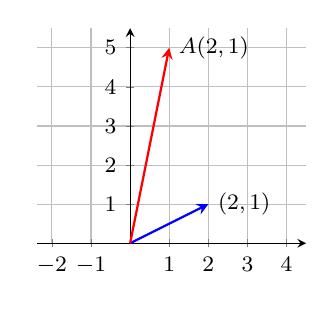
\begin{tikzpicture}[]
\begin{axis}[footnotesize,font=\footnotesize%,width=12em
    , axis equal , axis lines=middle,
    , grid, xmax=4.5,ymax=5.5 ]
    \addplot[blue,quiver={u=2,v=1},-stealth, thick] coordinates {(0,0)};
    \node[right] at (axis cs:2,1) {$(2,1)$};
    \addplot[red,quiver={u=1,v=5},-stealth, thick] coordinates {(0,0)};
    \node[right] at (axis cs:1,5) {$A(2,1)$};
\end{axis}
\end{tikzpicture}}%

Being the inverse, matrix~\(B\) `undoes' the action of matrix~\(A\)---as illustrated in the margin.
The first picture shows multiplication by~\(A\) transforms the vector~\((2,1)\) to the vector~\((1,5)\): \(A\footnotesize\begin{bmatrix} 2\\1 \end{bmatrix}=\begin{bmatrix} 1\\5 \end{bmatrix}\).
The second picture shows that multiplication by~\(B\) undoes the transform by~\(A\) because \(B\footnotesize\begin{bmatrix} 1\\5 \end{bmatrix}=\begin{bmatrix} 2\\1 \end{bmatrix}\) the original vector.
\marginpar{%
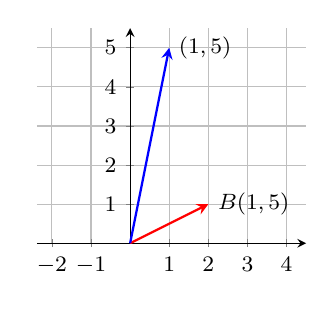
\begin{tikzpicture}[]
\begin{axis}[footnotesize,font=\footnotesize%,width=12em
    , axis equal, axis lines=middle,
    , grid, xmax=4.5,ymax=5.5 ]
    \addplot[red,quiver={u=2,v=1},-stealth, thick] coordinates {(0,0)};
    \node[right] at (axis cs:2,1) {$B(1,5)$};
    \addplot[blue,quiver={u=1,v=5},-stealth, thick] coordinates {(0,0)};
    \node[right] at (axis cs:1,5) {$(1,5)$};
\end{axis}
\end{tikzpicture}
}%
\end{solution}
\end{example}

The previous \autoref{eg:a2x2inv} shows at least one case when we can do some sort of matrix `division': that is, multiplying by~\(B\) is equivalent to `dividing' by~\(A\).
One restriction is that a clearly defined `division' only works for square matrices.
Part of the reason is because we need to be able to compute both~\(AB\) and~\(BA\).


\begin{definition}[inverse] \label{def:invertible} 
For every \(n\times n\) \idx{square matrix}~\(A\), an \bfidx{inverse} of~\(A\) is an \(n\times n\) matrix~\(B\) such that both \(AB=I_n\) and \(BA=I_n\)\,.
If such a matrix~\(B\) exists, then matrix~\(A\) is called \bfidx{invertible}.
\end{definition}

(By saying ``an inverse'' this definition allows for many inverses, but \autoref{thm:uninv} establishes that the inverse is unique.)

\begin{example} \label{eg:a3x3inv}
%A=round(randn(3,3)*5),B=inv(A)
Show that matrix
\begin{equation*}
B=\begin{bmatrix} 0&-\frac14&-\frac18\\\frac32&1&\frac78\\ \frac12&\frac14&\frac38 \end{bmatrix}
\text{ is an inverse of }
A=\begin{bmatrix} 1&-1&5\\-5&-1&3\\2&2&-6 \end{bmatrix}.
\end{equation*}

\begin{solution} 
First compute 
\begin{align*}
&AB=\begin{bmatrix} 1&-1&5\\-5&-1&3\\2&2&-6 \end{bmatrix}
\begin{bmatrix} 0&-\frac14&-\frac18\\\frac32&1&\frac78\\ \frac12&\frac14&\frac38 \end{bmatrix}
\\&=\footnotesize\let\cdt\cdot\def\cdot{\!\cdt\!}%squeeze it
\begin{bmatrix} 
1\cdot0 -1\cdot\frac32 +5\cdot\frac12&
1\cdot(-\frac14) -1\cdot1 +5\cdot\frac14&
1\cdot(-\frac18) -1\cdot\frac78 +5\cdot\frac38\\
-5\cdot0 -1\cdot\frac32 +3\cdot\frac12&
-5\cdot(-\frac14) -1\cdot1 +3\cdot\frac14&
-5\cdot(-\frac18) -1\cdot\frac78 +3\cdot\frac38\\
2\cdot0 +2\cdot\frac32 -6\cdot\frac12&
2\cdot(-\frac14) +2\cdot1 -6\cdot\frac14&
2\cdot(-\frac18) +2\cdot\frac78 -6\cdot\frac38
\end{bmatrix}
\\&=\begin{bmatrix} 1&0&0\\ 0&1&0\\ 0&0&1 \end{bmatrix}=I_3\,.
\end{align*}
Second compute
\begin{align*}
&BA=
\begin{bmatrix} 0&-\frac14&-\frac18\\\frac32&1&\frac78\\ \frac12&\frac14&\frac38 \end{bmatrix}
\begin{bmatrix} 1&-1&5\\-5&-1&3\\2&2&-6 \end{bmatrix}
\\&=\footnotesize\let\cdt\cdot\def\cdot{\!\cdt\!}%squeeze it
\begin{bmatrix}  
      0\cdot1 -\frac14\cdot(-5) -\frac18\cdot2 &
      0\cdot(-1) -\frac14\cdot(-1) -\frac18\cdot2 &
      0\cdot5 -\frac14\cdot3 -\frac18\cdot(-6) \\
\frac32\cdot1 +1\cdot(-5) +\frac78\cdot2 &
\frac32\cdot(-1) +1\cdot(-1) +\frac78\cdot2 &
\frac32\cdot5 +1\cdot3 +\frac78\cdot(-6) \\
\frac12\cdot1 +\frac14\cdot(-5) +\frac38\cdot2 &
\frac12\cdot(-1) +\frac14\cdot(-1) +\frac38\cdot2 &
\frac12\cdot5 +\frac14\cdot3 +\frac38\cdot(-6) 
\end{bmatrix}
\\&=\begin{bmatrix} 1&0&0\\ 0&1&0\\ 0&0&1 \end{bmatrix}=I_3\,.
\end{align*}
Since both of these products are the identity, then matrix~\(A\) is invertible, and \(B\)~is an inverse of~\(A\).
\end{solution}
\end{example}




\begin{activity}
What value of~\(b\) makes the matrix \(\begin{bmatrix} -1&b\\1&2 \end{bmatrix}\) to be the inverse of
\(\begin{bmatrix} 2&3\\-1&-1 \end{bmatrix}\)?
% a=0+round(randn(2)*3),b=inv(a)
\actposs[4]{\(-3\)}{\(-2\)}{\(1\)}{\(3\)}
%\partswidth=5em
%\begin{parts}
%\item \(-3\)\actans
%\item \(-2\)
%\item \(1\)
%\item \(3\)
%\end{parts}
\end{activity}





But even among square matrices, there are many non-zero matrices which do not have an inverse!
A matrix which is not invertible is sometimes called a \bfidx{singular matrix}.
The next \autoref{sec:fisvd} further explores why some matrices do not have an inverse: the reason is associated with both \index{rcond()@\texttt{rcond()}}\verb|rcond| being zero (\autoref{pro:unisol}) and/or the so-called determinant being zero (\autoref{ch:ddm}).

\begin{example}[no inverse] \label{eg:no2x2inv}
Prove that the matrix
\begin{equation*}
A=\begin{bmatrix} 1&-2\\-3&6 \end{bmatrix}
\end{equation*}
does not have an inverse.
\begin{solution} 
Assume there is an inverse matrix
\begin{equation*}
B=\begin{bmatrix} a&b\\c&d \end{bmatrix}.
\end{equation*}
Then by \autoref{def:invertible} the product \(AB=I_2\); that is,
\begin{eqnarray*}
AB&=&\begin{bmatrix} 1&-2\\-3&6 \end{bmatrix}
\begin{bmatrix} a&b\\c&d \end{bmatrix}
\\&=&\begin{bmatrix} a-2c&b-2d\\-3a+6c&-3b+6d \end{bmatrix}
=\begin{bmatrix} 1&0\\0&1 \end{bmatrix}.
\end{eqnarray*}
The bottom-left entry in this matrix equality asserts \(-3a+6c=0\) which is \(-3(a-2c)=0\), that is, \(a-2c=0\)\,.
But the top-left entry in the matrix equality asserts \(a-2c=1\)\,.
Both of these equations involving~\(a\) and~\(c\) cannot be true simultaneously; therefore the assumption of an inverse must be incorrect.
This matrix~\(A\) does not have an inverse.
\end{solution}
\end{example}



\begin{theorem}[unique inverse] \label{thm:uninv} 
If \(A\) is an \idx{invertible} matrix, then its \idx{inverse} is unique (and denoted by~\(A^{-1}\)).
\end{theorem}
\begin{proof} 
We suppose there are two inverses, say \(B_1\) and~\(B_2\), and proceed to show they must be the same.
Since they are inverses, by \autoref{def:invertible} both
\(AB_1=B_1A=I_n\) and \(AB_2=B_2A=I_n\)\,.
Consequently, using associativity of matrix multiplication (\autoref{thm:pmma}),
\begin{equation*}
B_1=B_1I_n=B_1(AB_2)=(B_1A)B_2=I_nB_2=B_2\,.
\end{equation*}
That is, \(B_1=B_2\) and so the inverse is unique.
\end{proof}



In the elementary case of \(1\times1\) matrices, that is \(A=\begin{bmatrix} a_{11} \end{bmatrix}\), the inverse is simply the reciprocal of the entry, that is \(A^{-1}=\begin{bmatrix} 1/a_{11} \end{bmatrix}\) provided \(a_{11}\)~is non-zero.
The reason is that \(AA^{-1}=\begin{bmatrix} a_{11}\cdot\frac1{a_{11}} \end{bmatrix}=\begin{bmatrix} 1 \end{bmatrix}=I_1\) and  \(A^{-1}A=\begin{bmatrix} \frac1{a_{11}}\cdot a_{11} \end{bmatrix}=\begin{bmatrix} 1 \end{bmatrix}=I_1\)\,.

In the case of \(2\times2\) matrices the inverse is a little more complicated, but should be remembered.
(For larger sized matrices, any direct general formulas for an inverse are too complicated to remember.)

\begin{theorem}[\(2\times2\) inverse] \label{thm:2x2det} 
Let \(2\times2\) matrix \(A=\begin{bmatrix} a&b\\c&d \end{bmatrix}\). Then \(A\)~is \idx{invertible} if the \bfidx{determinant} \(ad-bc\neq0\)\,, in which case
\begin{equation}
A^{-1}=\frac1{ad-bc}\begin{bmatrix} d&-b\\-c&a \end{bmatrix}.
\label{eq:2x2inv}
\end{equation}
If the determinant \(ad-bc=0\)\,, then \(A\)~is not \idx{invertible}.
\end{theorem}

\begin{example} \label{eg:}
\begin{enumerate}
\item Recall that \autoref{eg:a2x2inv} verified that
\begin{equation*}
B=\begin{bmatrix} -3&1\\-4&1 \end{bmatrix}
\text{ is an inverse of }
A=\begin{bmatrix} 1&-1\\4&-3 \end{bmatrix}.
\end{equation*}
Formula~\eqref{eq:2x2inv} gives this inverse from the matrix~\(A\): its elements are \(a=1\)\,, \(b=-1\)\,, \(c=4\) and \(d=-3\) so the determinant \(ad-bc=1\cdot(-3)-(-1)\cdot4=1\) and hence formula~\eqref{eq:2x2inv} derives the inverse
\begin{equation*}
A^{-1}=\frac11\begin{bmatrix} -3&-(-1)\\-4&1 \end{bmatrix}
=\begin{bmatrix} -3&1\\-4&1 \end{bmatrix}=B\,.
\end{equation*}

\item Further, recall \autoref{eg:no2x2inv} proved there is no inverse for matrix
\begin{equation*}
A=\begin{bmatrix} 1&-2\\-3&6 \end{bmatrix}.
\end{equation*}
\autoref{thm:2x2det} also establishes this matrix is not invertible because the matrix determinant \(ad-bc=1\cdot6-(-2)\cdot(-3)=6-6=0\)\,. 
\end{enumerate}
\end{example}




\begin{activity}
Which of the following matrices is invertible?
\actposs{\(\begin{bmatrix} 0&-3\\4&-2 \end{bmatrix}\)}
{\(\begin{bmatrix} -2&-1&4\\3&1&1 \end{bmatrix}\)}
{\(\begin{bmatrix} -2&1\\4&-2 \end{bmatrix}\)}
{\(\begin{bmatrix} -4&-2\\2&2\\-3&1 \end{bmatrix}\)}
%\begin{parts}
%\item \(\begin{bmatrix} -2&-1&4\\3&1&1 \end{bmatrix}\)
%\item \(\begin{bmatrix} 0&-3\\4&-2 \end{bmatrix}\)\actans
%\item \(\begin{bmatrix} -2&1\\4&-2 \end{bmatrix}\)
%\item \(\begin{bmatrix} -4&-2\\2&2\\-3&1 \end{bmatrix}\)
%\end{parts}
\end{activity}



\begin{proof} 
To prove \autoref{thm:2x2det}, first show the given~\(A^{-1}\) satisfies \autoref{def:invertible} when the determinant \(ad-bc\neq 0\) (and using associativity of scalar-matrix multiplication, \autoref{thm:pmmc}).
For the proposed~\(A^{-1}\), on the one hand,
\begin{eqnarray*}
A^{-1}A&=&\frac1{ad-bc}\begin{bmatrix} d&-b\\-c&a \end{bmatrix}
\begin{bmatrix} a&b\\c&d \end{bmatrix}
\\&=&\frac1{ad-bc}\begin{bmatrix} da-bc&db-bd\\-ca+ac&-cb+ad \end{bmatrix}
\\&=&\begin{bmatrix} 1&0\\0&1 \end{bmatrix}=I_2\,.
\end{eqnarray*}
On the other hand,
\begin{eqnarray*}
AA^{-1}&=&
\begin{bmatrix} a&b\\c&d \end{bmatrix}\begin{bmatrix} d&-b\\-c&a \end{bmatrix}\frac1{ad-bc}
\\&=&\begin{bmatrix} ad-bc&-ab+ba\\cd-dc&-cb+da \end{bmatrix}\frac1{ad-bc}
\\&=&\begin{bmatrix} 1&0\\0&1 \end{bmatrix}=I_2\,.
\end{eqnarray*}
By uniqueness (\autoref{thm:uninv}), equation~\eqref{eq:2x2inv} is the only inverse when \(ad-bc\neq 0\)\,.

Now eliminate the case when \(ad-bc=0\)\,.
If an inverse exists, say~\(X\), then it must satisfy \(AX=I_2\).
The top-left entry of this matrix equality requires \(ax_{11}+bx_{21}=1\)\,, whereas the bottom-left equality requires \(cx_{11}+dx_{21}=0\)\,.
Regard these as a system of two linear equations for the as yet unknowns \(x_{11}\) and~\(x_{21}\): from \(d\times\)~the first subtract \(b\times\)~the second to deduce that an inverse requires
\(dax_{11}+dbx_{21}-bcx_{11}-bdx_{21}=d\cdot1-b\cdot0\)\,.
By cancellation and factorising~\(x_{11}\), this equation then requires \((ad-bc)x_{11}=d\)\,.
But the determinant is zero, so this equation requires \(0\cdot x_{11}=d\)\,.
\begin{itemize}
\item If element~\(d\) is non-zero, then this equation cannot be satisfied and hence no inverse can be found.
\item Otherwise, if \(d\) is zero, then any~\(x_{11}\) satisfies this equation so if there is an inverse then there would be an infinite number of inverses (through the free variable~\(x_{11}\)).
But this contradicts the uniqueness \autoref{thm:uninv} so an inverse cannot exist in this case either.
\end{itemize}
That is, if the determinant \(ad-bc=0\)\,, then the \(2\times2\) matrix is not invertible.
\end{proof}



\begin{quoted}{\parbox[t]{0.5\linewidth}{G.~E. Forsythe and C.~B. Moler, 1967 \cite[p.261]{Higham1996}}}
Almost anything you can do with \(A^{-1}\) can be done without it.
\end{quoted}


\paragraph{Computer considerations} 
Except for easy cases such as \(2\times2\) matrices, we rarely explicitly compute the \idx{inverse} of a matrix.
Computationally there are (almost) always better ways such as the \script\ operation~\verb|A\b| of \autoref{pro:unisol}.
The \idx{inverse} is a crucial theoretical device, rarely a practical computational tool.


The following \autoref{thm:invuniqsol} is an example: for a system of linear equations the theorem connects the existence of a unique solution to the invertibility of the matrix of coefficients.
Further, \autoref{sec:svdsgs} connects solutions to the \verb|rcond| invoked by \autoref{pro:unisol}.
Although in theoretical statements we write expressions like \(\xv=A^{-1}\bv\)\,,
practically, once we know a solution exists (\verb|rcond| is acceptable), we generally compute a solution without ever constructing~\(A^{-1}\).



\begin{theorem} \label{thm:invuniqsol} 
If \(A\) is an \idx{invertible} \(n\times n\) matrix, then the system of \idx{linear equation}s \(A\xv=\bv\) has the \idx{unique solution} \(\xv=A^{-1}\bv\) for every \(\bv\) in~\(\RR^n\).
\end{theorem}

One consequence is the following: if a system of linear equations has no solution or an infinite number of solutions (\autoref{thm:fred}), then this theorem establishes that the matrix of the system is not invertible.

\begin{proof} 
The proof has two parts: first showing \(\xv=A^{-1}\bv\) is a solution, and second showing that there are no others.
First,  try \(\xv=A^{-1}\bv\) and use associativity (\autoref{thm:pmma}) and the inverse \autoref{def:invertible}:
\begin{equation*}
A\xv=A(A^{-1}\bv)=(AA^{-1})\bv=I_n\bv=\bv\,.
\end{equation*}
Second, suppose~\yv\ is any solution, that is, \(A\yv=\bv\)\,.
Multiply both sides by the inverse~\(A^{-1}\), and again use associativity and the definition of the inverse, to deduce
\begin{eqnarray*}
A^{-1}(A\yv)=A^{-1}\bv
&\implies& (A^{-1}A)\yv=\xv
\\&\implies& I_n\yv=\xv
\\&\implies& \yv=\xv\,.
\end{eqnarray*}
Since any solution~\yv\ has to be the same as~\xv, \(\xv=A^{-1}\bv\) is the unique solution.
\end{proof}





\begin{example} \label{eg:}
Use the matrices of Examples~\ref{eg:a2x2inv}, \ref{eg:a3x3inv} and~\ref{eg:no2x2inv} to decide whether each of the following systems have a unique solution, or not.
\begin{parts}
\item \(\begin{cases}
x-y=4\,,\\4x-3y=3\,.
\end{cases}\)
\item \(\begin{cases}
u-v+5w=2\,,\\ -5u-v+3w=5\,,\\ 2u+2v-6w=1\,.
\end{cases}\)
\item \(\begin{cases}
r-2s=-1\,,\\-3r+6s=3\,.
\end{cases}\)
\end{parts}
\begin{solution} 
\begin{enumerate}
\item A matrix for this system is \(\footnotesize\begin{bmatrix} 1&-1\\4&-3 \end{bmatrix}\) which \autoref{eg:a2x2inv} shows has an inverse.  
\autoref{thm:invuniqsol} then assures us the system has a unique solution.
\item A matrix for this system is \(\footnotesize\begin{bmatrix} 1&-1&5\\-5&-1&3\\2&2&-6 \end{bmatrix}\) which \autoref{eg:a3x3inv} shows has an inverse.  
\autoref{thm:invuniqsol} then assures us the system has a unique solution.
\item A matrix for this system is \(\footnotesize\begin{bmatrix} 1&-2\\-3&6 \end{bmatrix}\) which \autoref{eg:no2x2inv} shows is not invertible.  
\autoref{thm:invuniqsol} then assures us the system does not have a unique solution.
By \autoref{thm:fred} there may be either no solution or an infinite number of solutions---the matrix alone does not tell us which.
\end{enumerate}
\end{solution}
\end{example}






\begin{example} \label{eg:}
Given the following information about solutions of systems of linear equations, write down if the matrix associated with each system is invertible, or not, or there is not enough given information to decide.  Give reasons.
\begin{parts}
\item A general solution is \((1,-5,0,3)\).
\item A general solution is \((3,-5+3t,3-t,-1)\).
\item A solution of a system is \((-3/2,-2,-\pi,2,-4)\).
\item A solution of a homogeneous system is \((1,2,-8)\).
\end{parts}
\begin{solution} 
\begin{enumerate}
\item Since the solution is unique, the matrix in the system must be invertible.
\item This solution has an apparent free parameter,~\(t\), and so there are many solutions which implies the matrix is not invertible.
\item Not enough information is given as we do not know whether there are any more solutions.
\item Since a homogeneous system always has~\ov\ as a solution (\autoref{sec:3pns}), then we know that there are at least two solutions to the system, and hence the matrix is not invertible.
\end{enumerate}
\end{solution}
\end{example}




Recall from \autoref{sec:moaa} the properties of scalar multiplication, matrix powers, transpose, and their computation (\autoref{tbl:mtlbops}).
The next theorem incorporates the inverse into this suite of properties.


\begin{theorem}[properties of the inverse] \label{thm:invprop} 
Let \(A\) and~\(B\) be \idx{invertible} matrices of the same size, then:
\begin{enumerate}
\item\label{thm:invpropa}  matrix \(A^{-1}\) is invertible and \((A^{-1})^{-1}=A\)\,;
\item\label{thm:invpropb} if scalar \(c\neq0\)\,, then matrix~\(cA\) is invertible and \((cA)^{-1}=\frac1cA^{-1}\);
\item\label{thm:invpropc} 
matrix \(AB\) is invertible\begin{aside}
Remember the reversed order in the identity $(AB)^{-1}=B^{-1}A^{-1}$.
\end{aside} 
and \((AB)^{-1}=B^{-1}A^{-1}\);
\item\label{thm:invpropd} matrix \(\tr A\) is invertible and \((\tr A)^{-1}=\tr{(A^{-1})}\);
\item\label{thm:invprope} matrices \(A^p\) are invertible for all \(p=1,2,3,\ldots\) and \((A^p)^{-1}=(A^{-1})^p\).
\end{enumerate}
\end{theorem}


\begin{proof} 
Three parts are proved, and two are left as exercises.
\begin{description}
\item[\ref{thm:invpropa}]
By \autoref{def:invertible} the matrix~\(A^{-1}\) satisfies \(A^{-1}A=AA^{-1}=I\)\,.
But also by \autoref{def:invertible} this is exactly the identities we need to assert that matrix~\(A\) is the inverse of matrix~\((A^{-1})\).
Hence \(A=(A^{-1})^{-1}\).

\item[\ref{thm:invpropc}]
Test that \(B^{-1}A^{-1}\) has the required properties for the inverse of~\(AB\).
First, by associativity (\autoref{thm:pmma}) and multiplication by the identity (\autoref{thm:pmmd})
\begin{equation*}
(B^{-1}A^{-1})(AB)
=B^{-1}(A^{-1}A)B
=B^{-1}IB
=B^{-1}B
=I\,.
\end{equation*}
Second, and similarly
\begin{equation*}
(AB)(B^{-1}A^{-1})
=A(BB^{-1})A^{-1}
=AIA^{-1}
=AA^{-1}
=I\,.
\end{equation*}
Hence by \autoref{def:invertible} and the uniqueness \autoref{thm:uninv}, matrix~\(AB\) is invertible and \(B^{-1}A^{-1}\) is the inverse.

\item[\ref{thm:invprope}]
Prove by induction and use~\autoref{thm:invpropc}.
\begin{itemize}
\item For the case of exponent \(p=1\)\,, \((A^1)^{-1}=(A)^{-1}=A^{-1}=(A^{-1})^1\) and so the identity holds.
\item For any integer exponent \(p\geq2\)\,, assume the identity \((A^{p-1})^{-1}=(A^{-1})^{p-1}\).
Consider 
\begin{eqnarray*}
(A^p)^{-1}&=&(AA^{p-1})^{-1}\quad(\text{by power law \autoref{thm:pmmg}})
\\&=&(A^{p-1})^{-1}A^{-1}\quad(\text{\autoref{thm:invpropc}, }B=A^{p-1})
\\&=&(A^{-1})^{p-1}A^{-1}\quad(\text{by inductive assumption})
\\&=&(A^{-1})^p \quad(\text{by power law \autoref{thm:pmmg}}).
\end{eqnarray*}
\item By induction, the identity \((A^{p})^{-1}=(A^{-1})^{p}\) holds for exponents \(p=1,2,3,\ldots\)\,.
\end{itemize}
 
\end{description}
\end{proof}




\begin{activity}
The matrix \(\begin{bmatrix} 3&-5\\4&-7 \end{bmatrix}\) has inverse \(\begin{bmatrix} 7&-5\\4&-3 \end{bmatrix}\).
\begin{itemize}
\item What is the inverse of the matrix \(\begin{bmatrix} 6&-10\\8&-14 \end{bmatrix}\)?
% for i=1:999, a=0+round(randn(2)*4); if abs(det(a))==1, a=a, break,end, end
\actposs{\(\begin{bmatrix} 3.5&-2.5\\2&-1.5 \end{bmatrix}\)}
{\(\begin{bmatrix} 14&-10\\8&-3 \end{bmatrix}\)}
{\(\begin{bmatrix} 3.5&2\\-2.5&-1.5 \end{bmatrix}\)}
{\(\begin{bmatrix} 7&4\\-5&-3 \end{bmatrix}\)}
%\begin{parts}
%\item \(\begin{bmatrix} 14&-10\\8&-3 \end{bmatrix}\)
%\item \(\begin{bmatrix} 3.5&-2.5\\2&-1.5 \end{bmatrix}\)
%\item \(\begin{bmatrix} 3.5&2\\-2.5&-1.5 \end{bmatrix}\)
%\item \(\begin{bmatrix} 7&4\\-5&-3 \end{bmatrix}\)
%\end{parts}
\item Further, which of the above is the inverse of \(\begin{bmatrix} 3&4\\-5&-7 \end{bmatrix}\)?
\end{itemize}
\end{activity}





\begin{definition}[non-positive powers] \label{def:invpow} 
For every \idx{invertible} matrix~\(A\), define \(A^0:=I\) and for every positive integer~\(p\) define \(A^{-p}:=(A^{-1})^p\) (or by \autoref{thm:invprope} equivalently as~\((A^p)^{-1}\)).
\end{definition}

\begin{example} \label{eg:a2x2negp}
Recall from \autoref{eg:a2x2inv} that matrix
\begin{equation*}
A=\begin{bmatrix} 1&-1\\4&-3 \end{bmatrix}
\text{ has inverse }
A^{-1}=\begin{bmatrix} -3&1\\-4&1 \end{bmatrix}.
\end{equation*}
Compute \(A^{-2}\) and~\(A^{-4}\).
\begin{solution} 
From \autoref{def:invpow},
\begin{eqnarray*}
A^{-2}&=&(A^{-1})^2
=\begin{bmatrix} -3&1\\-4&1 \end{bmatrix}\begin{bmatrix} -3&1\\-4&1 \end{bmatrix}
=\begin{bmatrix} 5&-2\\8&-3 \end{bmatrix},
\\
A^{-4}&=&(A^{-1})^4
=\big[(A^{-1})^2\big]^2
\\&=&\begin{bmatrix} 5&-2\\8&-3 \end{bmatrix}\begin{bmatrix} 5&-2\\8&-3 \end{bmatrix}
=\begin{bmatrix} 9&-4\\16&-7 \end{bmatrix},
\end{eqnarray*}
upon using one of the power laws of \autoref{thm:pmmg}.
\end{solution}
\end{example}



\begin{activity}
\autoref{eg:a2x2negp} gives the inverse of a matrix~\(A\) and determines~\(A^{-2}\): what is~\(A^{-3}\)?
\actposs{\(\begin{bmatrix} -7&3\\-12&5 \end{bmatrix}\)}
{\(\begin{bmatrix} 3&-7\\5&-12 \end{bmatrix}\)}
{\(\begin{bmatrix} -7&-12\\3&5 \end{bmatrix}\)}
{\(\begin{bmatrix} 3&5\\-7&-12 \end{bmatrix}\)}
%\begin{parts}
%\item \(\begin{bmatrix} -7&3\\-12&5 \end{bmatrix}\)\actans
%\item \(\begin{bmatrix} 3&-7\\5&-12 \end{bmatrix}\)
%\item \(\begin{bmatrix} -7&-12\\3&5 \end{bmatrix}\)
%\item \(\begin{bmatrix} 3&5\\-7&-12 \end{bmatrix}\)
%\end{parts}
\end{activity}




\begin{example}[predict the past] \label{eg:invph}
Recall \autoref{eg:matasp} introduced how to use a \idx{Leslie matrix} to predict the future population of an animal.
If \(\xv=(60,70,20)\) is the current number of pups, juveniles, and mature females respectively, then by the modelling the predicted population numbers after a year is \(\xv'=L\xv\), after two years is \(\xv''=L\xv'=L^2\xv\), and so on.
In these formulas, and for this example, the Leslie matrix
\begin{equation*}
L=\begin{bmatrix} 0&0&4\\\frac12&0&0\\0&\frac13&\frac13 \end{bmatrix},
\quad\text{which has inverse }L^{-1}=\begin{bmatrix} 0&2&0\\-\frac14&0&3\\\frac14&0&0 \end{bmatrix}.
\end{equation*} 
Assume the same rule applies for earlier years.
\begin{itemize}
\item Letting the population numbers a year ago be denoted by~\(\xv^-\) then by the modelling the current population \(\xv=L\xv^-\).
Multiply by the inverse of~\(L\): \(L^{-1}\xv=L^{-1}L\xv^-=\xv^-\); that is, the population a year before the current is \(\xv^-=L^{-1}\xv\).
\item Similarly, letting the population numbers two years ago be denoted by~\(\xv^=\) then  by the modelling \(\xv^-=L\xv^=\) and multiplication by~\(L^{-1}\) gives \(\xv^==L^{-1}\xv^-=L^{-1}L^{-1}\xv=L^{-2}\xv\).
\item One more year earlier, letting the population numbers two years ago be denoted by~\(\xv^\equiv\) then  by the modelling \(\xv^==L\xv^\equiv\) and multiplication by~\(L^{-1}\) gives \(\xv^\equiv=L^{-1}\xv^==L^{-1}L^{-2}\xv=L^{-3}\xv\).
\end{itemize}
Hence use the inverse powers of~\(L\) to predict the earlier history of the population of female animals in the given example: but first verify the given inverse is correct.
\begin{solution} 
Verify the given inverse by evaluating (showing only non-zero terms in a sum)
\begin{eqnarray*}
LL^{-1}&=&
\begin{bmatrix} 0&0&4\\\frac12&0&0\\0&\frac13&\frac13 \end{bmatrix}
\begin{bmatrix} 0&2&0\\-\frac14&0&3\\\frac14&0&0 \end{bmatrix}
\\&=&
\begin{bmatrix} 4\cdot\frac14&0&0\\
0&\frac12\cdot2&0\\
\frac13\cdot(-\frac14)+\frac13\cdot\frac14&0&\frac13\cdot3 \end{bmatrix}
\\&=&\begin{bmatrix} 1&0&0\\0&1&0\\0&0&1 \end{bmatrix}=I_3\,,
\\L^{-1}L&=&\begin{bmatrix} 0&2&0\\-\frac14&0&3\\\frac14&0&0 \end{bmatrix}
\begin{bmatrix} 0&0&4\\\frac12&0&0\\0&\frac13&\frac13 \end{bmatrix}
\\&=&\begin{bmatrix} 2\frac12&0&0\\
0&3\cdot\frac13&-\frac14\cdot4+3\cdot\frac13\\
0&0&\frac14\cdot4 \end{bmatrix}
\\&=&\begin{bmatrix} 1&0&0\\0&1&0\\0&0&1 \end{bmatrix}=I_3\,.
\end{eqnarray*}
Hence the given \(L^{-1}\) is indeed the inverse.
For the current population \(\xv=(60,70,20)\), now use the inverse to compute earlier populations.
\begin{itemize}
\item The population of females one year ago was
\begin{equation*}
\xv^-=L^{-1}\xv
=\begin{bmatrix} 0&2&0\\-\frac14&0&3\\\frac14&0&0 \end{bmatrix}
\begin{bmatrix} 60\\70\\20 \end{bmatrix}
=\begin{bmatrix} 140\\45\\15 \end{bmatrix}.
\end{equation*}
That is, there were 140~pups, 45~juveniles, and 15~mature females.
\item Computing the square of the inverse
\begin{equation*}
L^{-2}=(L^{-1})^2
=\begin{bmatrix} 0&2&0\\-\frac14&0&3\\\frac14&0&0 \end{bmatrix}^2
=\begin{bmatrix} -\frac12&0&6\\
\frac34&-\frac12&0\\
0&\frac12&0 \end{bmatrix},
\end{equation*}
we predict the population of females two years ago was
\begin{equation*}
\xv^==L^{-2}\xv
=\begin{bmatrix} -\frac12&0&6\\
\frac34&-\frac12&0\\
0&\frac12&0 \end{bmatrix}
\begin{bmatrix} 60\\70\\20 \end{bmatrix}
=\begin{bmatrix} 90\\10\\35 \end{bmatrix}.
\end{equation*}
\item Similarly, computing the cube of the inverse
\begin{equation*}
L^{-3}=L^{-2}L^{-1}=\cdots
=\begin{bmatrix} \frac32&-1&0\\
\frac18&\frac32&-\frac32\\
-\frac18&0&\frac32 \end{bmatrix},
\end{equation*}
we predict the population of females three years ago was
\begin{equation*}
\xv^\equiv=L^{-3}\xv
=\begin{bmatrix} \frac32&-1&0\\
\frac18&\frac32&-\frac32\\
-\frac18&0&\frac32 \end{bmatrix}
\begin{bmatrix} 60\\70\\20 \end{bmatrix}
=\begin{bmatrix} 20\\82.5\\22.5 \end{bmatrix}.
\end{equation*}
\end{itemize}
(Predicting half animals in this last calculation is because the modelling only deals with average numbers, not exact numbers.)
\end{solution}
\end{example}

\begin{example} \label{eg:}
As an alternative to the hand calculations of \autoref{eg:invph}, predict earlier populations by computing in \script\ without ever explicitly finding the inverse or powers of the inverse.
The procedure is to solve the linear system \(L\xv^-=\xv\) for the population~\(\xv^-\) a year ago, and then similarly solve \(L\xv^==\xv^-\), \(L\xv^\equiv=\xv^=\), and so on.
\begin{solution} 
Execute
\setbox\ajrqrbox\hbox{\qrcode{% predict history
L=[0 0 4;1/2 0 0;0 1/3 1/3]
x=[60;70;20]
rcond(L)
xm=L\slosh x
xmm=L\slosh xm
xmmm=L\slosh xmm
}}%
\marginpar{\usebox{\ajrqrbox}}%
\begin{verbatim}
L=[0 0 4;1/2 0 0;0 1/3 1/3]
x=[60;70;20]
rcond(L)
xm=L\x
xmm=L\xm
xmmm=L\xmm
\end{verbatim}
Since \verb|rcond| is~\(0.08\) (good by \autoref{pro:unisol}), this code uses~\verb|L\| to solve the linear systems and confirm the population of females in previous years is as determined by \autoref{eg:invph}, namely
\begin{equation*}
\verb|xm|=\begin{bmatrix} 140 \\ 45 \\ 15 \end{bmatrix},\quad
\verb|xmm|=\begin{bmatrix} 90 \\ 10 \\ 35 \end{bmatrix},\quad
\verb|xmmm|=\begin{bmatrix} 20 \\ 82.5 \\ 22.5 \end{bmatrix}.
\end{equation*} 
\end{solution}
\end{example}













\subsection{Diagonal matrices stretch and shrink}
\label{sec:dmd}
\index{diagonal matrix|(}

Recall that the identity matrices are zero except for a diagonal of ones from the top-left to the bottom-right of the matrix.
Because of the nature of matrix multiplication it is this diagonal that is special.
Because of the special nature of this diagonal, this section explores matrices which are zero except for the numbers (not generally ones) in the top-left to bottom-right diagonal.

\begin{example} \label{eg:4diag}
That is, this section explores the nature of so-called diagonal matrices such as
\begin{equation*}
%I_n,\quad
\begin{bmatrix} 3&0\\0&2 \end{bmatrix},\quad
\begin{bmatrix} 0.58&0&0\\0&-1.61&0\\0&0&2.17 \end{bmatrix},\quad
\begin{bmatrix} \pi&0&0\\0&\sqrt3&0\\0&0&0 \end{bmatrix}.
\end{equation*}
We use the term {diagonal matrix} to also include non-square matrices such as
\begin{equation*}
\begin{bmatrix} -\sqrt2&0\\0&\frac12\\0&0 \end{bmatrix},\quad
\begin{bmatrix} 1&0&0&0&0\\0&\pi&0&0&0\\0&0&e&0&0 \end{bmatrix}.
\end{equation*}
The term diagonal matrix does \emph{not} describe matrices such as
\begin{equation*}
\begin{bmatrix} 0&0&1\\0&2&0\\-\frac12&0&0  \end{bmatrix}
,\quad\text{and}\quad
\begin{bmatrix} -0.17&0&0&0\\0&-4.22&0&0\\0&0&0&3.05 \end{bmatrix}.
\end{equation*}
\end{example}

Amazingly, the singular value decomposition of \autoref{sec:fisvd} proves that diagonal matrices lie at the very heart of the action of \emph{every} matrix.

\begin{definition}[diagonal matrix] \label{def:diag} 
For every \(m\times n\) matrix~\(A\), the \bfidx{diagonal entries} of~\(A\) are \(a_{11},a_{22},\ldots,a_{pp}\) where \(p=\min(m,n)\).
A matrix whose non-diagonal entries are all zero is called a \bfidx{diagonal matrix}.

For brevity we may write \index{diag}\(\diag(\hlist vn)\) to denote the \(n\times n\) square matrix with diagonal entries \hlist vn\,, or \(\diag_{m\times n}(\hlist vp)\) for an \(m\times n\) matrix with diagonal entries \hlist vp.
\end{definition}

\begin{example} \label{eg:} \sloppy
The five diagonal matrices of \autoref{eg:4diag} could equivalently be written as \(\diag(3,2)\), \(\diag(0.58,-1.61,2.17)\) \(\diag(\pi,\sqrt3,0)\), \(\diag_{3\times2}(-\sqrt2,\tfrac12)\) and \(\diag_{3\times5}(1,\pi,e)\), respectively.
\end{example}


Diagonal matrices may also have zeros on the diagonal, as well as the required zeros for the non-diagonal entries.


\needspace{9\baselineskip}
\begin{activity}
Which of the following matrices are not diagonal?
\actposs{\(\begin{bmatrix} 1&0&0
\\0&0&0
\\0&2&0
\\0&0&0 \end{bmatrix}\)}
{\(I_n\)}{\(O_n\)}
{\(\begin{bmatrix} 1&0&0&0
\\0&2&0&0
\\0&0&0&0 \end{bmatrix}\)}
%\begin{parts}
%\item \(I_n\)
%\item \(O_n\)
%\item \(\begin{bmatrix} 1&0&0&0
%\\0&2&0&0
%\\0&0&0&0 \end{bmatrix}\)
%\item \(\begin{bmatrix} 1&0&0
%\\0&0&0
%\\0&2&0
%\\0&0&0 \end{bmatrix}\)\actans
%\end{parts}
\end{activity}
  


\begin{table}
\caption{As well as the basics of \script\ listed in Tables~\ref{tbl:mtlbpre}, \ref{tbl:mtlbbasics} and~\ref{tbl:mtlbops},  we need these matrix operations.\index{Matlab@\textsc{Matlab}|textbf}\index{Octave|textbf}} \label{tbl:mtlbmops}
\hrule
\begin{minipage}{\linewidth}
\begin{itemize}
\item \index{diag()@\texttt{diag()}}\verb|diag(v)| where \verb|v| is a row/column vector of length~\(p\) generates the \(p\times p\) matrix 
\begin{equation*}
\diag(\hlist vp)=\begin{bmatrix} v_1&0&\cdots&0\\
0&v_2&&\vdots\\ \vdots&&\ddots\\ 0&\cdots&&v_p \end{bmatrix}.
\end{equation*}
%Whereas \verb|diag(v,m,n)| generates the \(m\times n\) matrix \(\diag_{m\times n}(\hlist v{\min(p,m,n)})\). % only in Octave

\item In \script\ (but not usually in algebra), \verb|diag| also does the opposite: for an \(m\times n\) matrix~\(A\) such that both \(m,n\geq2\)\,,  \verb|diag(A)| returns the (column) vector \((a_{11},a_{22},\ldots,a_{pp})\) of diagonal entries where the result vector length \(p=\min(m,n)\).

\item The dot operators \index{./@\texttt{./}}\verb|./| and~\index{.*@\texttt{.*}}\verb|.*| do element-by-element division and multiplication of two matrices\slash vectors of the same size.  For example, 
\begin{verbatim}
[5 14 33]./[5 7 3]=[1 2 11]
\end{verbatim}


\item \autoref{sec:asie} also needs to compute the logarithm of data: \index{log10()@\texttt{log10()}}\verb|log10(v)| finds the logarithm to base~\(10\) of each component of~\verb|v| and returns the results in a vector of the same size; \index{log()@\texttt{log()}}\verb|log(v)| does the same but for the natural logarithm (not \verb|ln(v)|).

\end{itemize}
\end{minipage}
\hrule
\end{table}




\subsubsection{Solve systems whose matrix is diagonal}

Solving a system of linear equations (\autoref{def:lineqn}) is particularly straightforward when the matrix of the system is diagonal.
Indeed much mathematics in both theory and applications is devoted to transforming a given problem so that the matrix appearing in the  system is diagonal (e.g., sections~\ref{sec:amss} and~\ref{sec:svdsgs}, and Chapters~\ref{ch:eesm} and~\ref{ch:gee}).

\begin{comment}
Here prepare for using the \svd, but also use diagonal matrices to reinforce the translation to/from matrix and symbolic forms, and to reinforce zero, one, many solutions.
\end{comment}%


\begin{example} \label{eg:}
Solve \begin{equation*}
\begin{bmatrix} 3&0\\0&2 \end{bmatrix}
\begin{bmatrix} x_1\\x_2 \end{bmatrix}
=\begin{bmatrix} 2\\-5 \end{bmatrix}
\end{equation*}
\begin{solution}
Algebraically this matrix-vector equation means
\begin{equation*}
\begin{cases} 3x_1+0x_2=2 \\ 0x_1+2x_2=-5\end{cases}
\iff
\begin{cases} 3x_1=2 \\ 2x_2=-5\end{cases}
\iff
\begin{cases} x_1=2/3 \\ x_2=-5/2\end{cases}
\end{equation*}
The solution is \(\xv=(2/3,-5/2)\).
Interestingly, the two components of this solution are firstly the~\(2\) on the right-hand side divided by the~\(3\) in the matrix, and secondly the~\(-5\) on the right-hand side divided by the~\(2\) in the matrix.
%\begin{equation*}
%\xv=\begin{bmatrix} \frac23\\-\frac52 \end{bmatrix}
%=\begin{bmatrix} \frac13&0\\0&\frac12 \end{bmatrix}
%\begin{bmatrix} 2\\-5 \end{bmatrix}.
%\end{equation*}
\end{solution}
\end{example}






\begin{example} \label{eg:a3x3inw}
Solve \begin{equation*}
\begin{bmatrix} 2&0&0\\0&\frac23&0\\0&0&-1 \end{bmatrix}
\begin{bmatrix} x_1\\x_2\\x_3 \end{bmatrix}
=\begin{bmatrix} b_1\\b_2\\b_3 \end{bmatrix}
\end{equation*}
\begin{solution}
Algebraically this equation means
\begin{equation*}
\begin{cases} 2x_1+0x_2+0x_3=b_1
\\0x_1+\frac23x_2+0x_3=b_2
\\0x_1+0x_2-1x_3=b_3\end{cases}
\iff
\begin{cases} 2x_1=b_1
\\\frac23x_2=b_2
\\-x_3=b_3\end{cases}
\iff
\begin{cases} x_1=\frac12b_1 \\ x_2=\frac32b_2 \\ x_3=-b_3\end{cases}.
\end{equation*}
The solution is 
\begin{equation*}
\xv=\begin{bmatrix} \frac12b_1 \\ \frac32b_2 \\ -b_3 \end{bmatrix},
\quad\text{rewritten as }
\xv=\begin{bmatrix} \frac12&0&0\\0&\frac32&0\\0&0&-1 \end{bmatrix}
\begin{bmatrix} b_1\\b_2\\b_3 \end{bmatrix}.
\end{equation*}
Consequently, by its uniqueness (\autoref{thm:uninv}), the inverse of the given diagonal matrix must be
\begin{equation*}
\begin{bmatrix} 2&0&0\\0&\frac23&0\\0&0&-1 \end{bmatrix}^{-1}
=\begin{bmatrix} \frac12&0&0\\0&\frac32&0\\0&0&-1 \end{bmatrix},
\end{equation*}
which interestingly is the diagonal of reciprocals of the given matrix.
\end{solution}
\end{example}




\begin{activity}
What is the solution to the system \(\begin{bmatrix} 0.4&0\\0&0.1 \end{bmatrix}\xv=\begin{bmatrix} 0.1\\-0.2 \end{bmatrix}\)?
\actposs[4]{\((\frac14,-2)\)}{\((4,-2)\)}{\((\frac14,-\frac12)\)}{\((4,-\frac12)\)}
%\partswidth=5em
%\begin{parts}
%\item \((4,-2)\)
%\item \((\frac14,-\frac12)\)
%\item \((4,-\frac12)\)
%\item \((\frac14,-2)\)\actans
%\end{parts}
\end{activity}



\begin{comment}
Diagonal matrices are `stretchers' in the coordinate directions, e.g.~the rack.  They also can reflect which changes orientation.  They are a first example of a {linear transform}.  Their inverse has to undo the stretching.
\end{comment}

\begin{theorem}[inverse of diagonal matrix] \label{thm:idm}
For every \(n\times n\) \idx{diagonal matrix}  \(D=\diag(\hlist dn)\), 
if all the diagonal entries are nonzero, \(d_{i}\neq 0\) for \(i=1,2,\ldots,n\)\,, then \(D\)~is \idx{invertible} and the inverse \(D^{-1}=\diag(1/d_{1},1/d_{2},\ldots,1/d_{n})\).
\end{theorem}
\begin{proof} 
Consider the matrix product 
%\begin{maxipage}
\begin{align*}&
\begin{bmatrix} d_1&0&\cdots&0
\\0&d_2&&0
\\\vdots&&\ddots&\vdots
\\0&0&\cdots&d_n \end{bmatrix}
\begin{bmatrix} \frac1{d_1}&0&\cdots&0
\\0&\frac1{d_2}&&0
\\\vdots&&\ddots&\vdots
\\0&0&\cdots&\frac1{d_n} \end{bmatrix}
\\&=
\footnotesize%squeeze it in
\begin{bmatrix} d_1\frac1{d_1}+0+\cdots+0
&d_10+0\frac1{d_1}+\cdots+0
&\cdots&d_10+0+\cdots+0\frac1{d_n}
\\0\frac1{d_1}+d_20+\cdots+0
&0+d_2\frac1{d_2}+\cdots+0
&&0+d_20+\cdots+0\frac1{d_n}
\\\vdots&&\ddots&\vdots
\\0\frac1{d_1}+0+\cdots+d_n0
&0+0\frac1{d_2}+\cdots+d_n0
&\cdots&0+0+\cdots+d_n\frac1{d_n} \end{bmatrix}
\\&=\begin{bmatrix} 1&0&\cdots&0
\\0&1&&0
\\\vdots&&\ddots&\vdots
\\0&0&\cdots&1 \end{bmatrix}=I_n.
\end{align*}
%\end{maxipage}
Similarly for the reverse product.
By \autoref{def:invertible}, \(D\)~is invertible with the given inverse.
\end{proof}

\begin{example} \label{eg:}
The previous \autoref{eg:a3x3inw} gave the inverse of a \(3\times3\) matrix.  
For the \(2\times2\) matrix \(D=\diag(3,2)=\begin{bmatrix} 3&0\\0&2 \end{bmatrix}\) the inverse is \(D^{-1}=\diag(\frac13,\frac12)=\begin{bmatrix} \frac13&0\\0&\frac12 \end{bmatrix}\).  Then the solution to
\begin{equation*}
\begin{bmatrix} 3&0\\0&2 \end{bmatrix}\xv
=\begin{bmatrix} 2\\-5 \end{bmatrix}
\quad\text{is }\xv=\begin{bmatrix} \frac13&0\\0&\frac12 \end{bmatrix}
\begin{bmatrix} 2\\-5 \end{bmatrix}=\begin{bmatrix} 2/3\\-5/2 \end{bmatrix}.
\end{equation*}
\end{example}


\begin{compute}
To solve the matrix-vector equation \(D\xv=\bv\) recognise that this equation means
\begin{eqnarray}&&
\begin{bmatrix} d_1&0&\cdots&0
\\0&d_2&&0
\\\vdots&&\ddots&\vdots
\\0&0&\cdots&d_n \end{bmatrix}
\begin{bmatrix} x_1\\x_2\\\vdots\\x_n \end{bmatrix}
=\begin{bmatrix} d_1x_1\\d_2x_2\\\vdots\\d_nx_n \end{bmatrix}
=\begin{bmatrix} b_1\\b_2\\\vdots\\b_n \end{bmatrix}
\nonumber\\&&\iff
\begin{cases} d_1x_1=b_1\\d_2x_2=b_2\\\vdots\\d_nx_n=b_n \end{cases}
\iff
\begin{cases} x_1=b_1/d_1\\x_2=b_2/d_2\\\vdots\\x_n=b_n/d_n \end{cases}
\label{eq:ddslin}
\end{eqnarray}
\begin{itemize}
\item Suppose you have a column vector~\verb|d| of the diagonal entries of~\(D\) and a column vector~\verb|b| of the \rhs; then compute a solution by, for example,
\setbox\ajrqrbox\hbox{\qrcode{% element by element division
d=[2;2/3;-1]
b=[1;2;3]
x=b./d
}}%
\marginpar{\usebox{\ajrqrbox\\[2ex]}}%
\begin{verbatim}
d=[2;2/3;-1]
b=[1;2;3]
x=b./d
\end{verbatim}
to find the answer \verb|[0.5;3;-3]|.
Here the \script\ operation~\verb|./| does  element-by-element division (\autoref{tbl:mtlbmops}).

\item When you have the diagonal matrix in full:  extract the diagonal elements into a column vector with \verb|diag()| (\autoref{tbl:mtlbmops});  then execute the element-by-element division; for example,
\setbox\ajrqrbox\hbox{\qrcode{% solve diagonal system
D=[2 0 0;0 2/3 0;0 0 -1]
b=[1;2;3]
x=b./diag(D)
}}%
\marginpar{\usebox{\ajrqrbox\\[2ex]}}%
\begin{verbatim}
D=[2 0 0;0 2/3 0;0 0 -1]
b=[1;2;3]
x=b./diag(D)
\end{verbatim}
\end{itemize}

%\begin{itemize}
%\item \verb|./| is component by component division.
%\item \verb|diag()| does one of two things:
%\begin{itemize}
%\item \verb|diag(d)| for row or \idx{column vector}~\(\dv\) in~\(\RR^n\) generates the \(n\times n\) \idx{diagonal matrix}~\(D\) with entries \(d_{ii}=d_i\) and zero elsewhere; whereas
%\item \verb|diag(A)| for \(m\times n\) matrix~\(A\) extracts the diagonal entries and forms a \idx{column vector} in~\(\RR^{\min(m,n)}\) whose \(i\)th~entry is~\(a_{ii}\).
%\end{itemize}
%\end{itemize}
\end{compute}


\subsubsection{But do not divide by zero} 
Dividing by zero is almost aways nonsense.
Instead use reasoning.
Consider solving \(D\xv=\bv\) for diagonal~\(D=\diag(\hlist dn)\) where \(d_n=0\) (and similarly for any others that are zero).
From~\eqref{eq:ddslin} we need to solve \(d_nx_n=b_n\)\,, which here is \(0\cdot x_n=b_n\)\,, that is, \(0=b_n\)\,. 
There are two cases: 
\begin{itemize}
\item if \(b_n\neq 0\)\,, then there is no solution; conversely
\item if \(b_n=0\)\,, then there is an infinite number of solutions as any~\(x_n\) satisfies \(0\cdot x_n=0\)\,.
\end{itemize}





\begin{example} \label{eg:}
Solve the two systems (the only difference is the last component on the \rhs)
\begin{equation*}
\begin{bmatrix} 2&0&0\\0&\frac23&0\\0&0&0 \end{bmatrix}
\begin{bmatrix} x_1\\x_2\\x_3 \end{bmatrix}
=\begin{bmatrix} 1\\2\\3 \end{bmatrix}
\quad\text{and }
\begin{bmatrix} 2&0&0\\0&\frac23&0\\0&0&0 \end{bmatrix}
\begin{bmatrix} x_1\\x_2\\x_3 \end{bmatrix}
=\begin{bmatrix} 1\\2\\0 \end{bmatrix}
\end{equation*}
\begin{solution}
Algebraically, the first system means
\begin{equation*}
\begin{array}{l} 2x_1+0x_2+0x_3=1
\\0x_1+\frac23x_2+0x_3=2
\\0x_1+0x_2+0x_3=3\end{array}
\iff
\begin{array}{l} 2x_1=1
\\\frac23x_2=2
\\0x_3=3\end{array}
.
\end{equation*}
There is no solution in the first case as there is no choice of~\(x_3\) such that \(0x_3=3\)\,.

Algebraically, the second system means
\begin{equation*}
\begin{array}{l} 2x_1+0x_2+0x_3=1
\\0x_1+\frac23x_2+0x_3=2
\\0x_1+0x_2+0x_3=0\end{array}
\iff
\begin{array}{l} 2x_1=1
\\\frac23x_2=2
\\0x_3=0\end{array}
.
\end{equation*}
In this second case we satisfy the equation \(0x_3=0\) with any~\(x_3\).
Hence there are an infinite number of solutions, namely \(\xv=(\frac12,3,t)\) for all~\(t\)---a free variable just as in Gauss--Jordan elimination (\autoref{pro:gje}).
\end{solution}
\end{example}




\subsubsection{Stretch or squash the unit square}

\begin{quoted}{\index{Hawking, Stephen}Stephen Hawking, 2005}
Equations are just the boring part of mathematics.  
I attempt to see things in terms of geometry.
\end{quoted}


%\begin{aside}
%This geometric interpretation prepares for the geometry of rotation by orthogonal matrices.
%\end{aside} 
Multiplication by matrices transforms shapes:
multiplication by diagonal matrices just stretches or squashes and/or reflects in the direction of the coordinate axes.
The next \autoref{sec:omr} introduces matrices that rotate.




\begin{example} \label{eg:}
Consider \(A=\diag(3,2)=\footnotesize\begin{bmatrix} 3&0\\0&2 \end{bmatrix}\). 
\marginpar{\TwoD3002}%
The marginal pictures shows this matrix stretches the (blue) unit square (drawn with a `roof') by a factor of three horizontally and two vertically (to the red). 
Recall that \((x_1,x_2)\) denotes the corresponding column vector.  
As seen in the corner points of the graphic in the margin,  \(A\times(1,0)=(3,0)\), \(A\times(0,1)=(0,2)\), \(A\times(0,0)=(0,0)\),  and \(A\times(1,1)=(3,2)\).   
The `roof' just helps us to track which corner goes where.

\marginpar{\TwoD{1/3}00{1/2}}%
The inverse \(A^{-1}=\diag(\frac13,\frac12)=\footnotesize\begin{bmatrix} \frac13&0\\0&\frac12 \end{bmatrix}\) undoes the stretching of the matrix~\(A\) by squashing in both the horizontal and vertical directions (from blue to red).  
\end{example}




\begin{example} \label{eg:}
Consider \(\diag(2,\frac23,-1)=\footnotesize\begin{bmatrix} 2&0&0\\0&\frac23&0\\0&0&-1 \end{bmatrix}\): 
the \idx{stereo pair} below illustrates how this diagonal matrix stretches in one direction, squashes in another, and reflects in the vertical.  
By multiplying the matrix by corner vectors \((1,0,0)\), \((0,1,0)\), \((0,0,1)\), and so on, we see that the blue unit cube (with `roof' and `door') maps to the red.
\begin{center}
\def\unithousesize{small}
\ThreeD{2}000{2/3}000{-1}
\end{center}
\end{example}

One great aspect of a diagonal matrix is that it is easy to separate its effects into each coordinate direction.  
For example, the above \(3\times3\) matrix is the same as the combined effects of the following three.
\begin{align*}
&\parbox[b]{0.35\linewidth}{\raggedright
\(\footnotesize\begin{bmatrix} 2&0&0\\0&1&0\\0&0&1 \end{bmatrix}\).  Stretch by a factor of two in the \(x_1\) direction.} &&
\ThreeD{2}000{1}000{1} 
\\&
\parbox[b]{0.35\linewidth}{\raggedright
\(\footnotesize\begin{bmatrix} 1&0&0\\0&\frac23&0\\0&0&1 \end{bmatrix}\).  Squash by a factor of \(2/3\) in the \(x_2\) direction.} &&
\ThreeD{1}000{2/3}000{1} 
\\&
\parbox[b]{0.35\linewidth}{\raggedright
\(\footnotesize\begin{bmatrix} 1&0&0\\0&1&0\\0&0&-1 \end{bmatrix}\).  Reflect in the  vertical \(x_3\) direction.} &&
\ThreeD{1}000{1}000{-1} 
\end{align*}





\begin{example} \label{eg:}
What diagonal matrix transforms the blue unit square to the red in the illustration in the margin? 
\marginpar{\TwoD{3/2}00{-1/2}}
\begin{solution} 
In the illustration, the horizontal is stretched by a factor of~\(3/2\), whereas the vertical is squashed by a factor of~\(1/2\), and reflected (minus sign). 
Hence the matrix is
\(\diag(\frac32,-\frac12)=\footnotesize\begin{bmatrix} \frac32&0\\0&-\frac12 \end{bmatrix}\).
\end{solution}
\end{example}




\begin{activity}
Which of the following diagrams represents the transformation from the (blue) unit square to the (red) rectangle by the matrix \(\diag(-1.3,0.7)\)?
\actposs{\TwoD{-1.3}00{0.7}}
{\TwoD{-0.7}00{1.3}}
{\TwoD{0.7}00{-1.3}}
{\TwoD{1.3}00{-0.7}}
%\begin{parts}
%\item \TwoD{-0.7}00{1.3}
%\item \TwoD{0.7}00{-1.3}
%\item \TwoD{-1.3}00{0.7}
%\item \TwoD{1.3}00{-0.7}
%\end{parts}
\end{activity}




\paragraph{Some diagonal matrices rotate}
Now consider the transformation of multiplying by matrix \(\footnotesize\begin{bmatrix} -1&0\\0&-1 \end{bmatrix}\):
\marginpar{\TwoD{-1}00{-1}}%
the two reflections of this diagonal matrix, the two~\(-1\)s, have  the same effect as one rotation, here by~\(180^\circ\), as shown to the left.
Matrices that rotate are incredibly useful and is the topic of the next \autoref{sec:omr}.





\subsubsection{Sketch convenient coordinates}
One of the fundamental principles of applying mathematics in science and engineering
is that the real world---nature---does its thing irrespective of our mathematical description.
\begin{aside}
This optional subsubsection is a preliminary to diagonalisation.
\end{aside}%
Hence we often simplify our mathematical description of real world applications by choosing a coordinate system to suit its nature.
That is, although this book (almost) always draws the \(x\) or \(x_1\)~axis horizontally, and the \(y\) or \(x_2\)~axis vertically, in applications it is often better to draw the axes in some other  directions---directions which are convenient for the application.
This example illustrates the principle.

\begin{example} \label{eg:}
Consider the transformation shown in the margin (it might arise from the deformation of some material and we need to know the internal stretching and shrinking to predict failure).
\marginpar{\TwoDx{1.04}{-0.72}{-0.72}{1.46}{}}%
The drawing has no coordinate axes shown because it supposed to be some transformation in nature. 
Now we impose on nature our mathematical description.
Draw approximate coordinate axes, with origin at the common point at the lower-left corner, so the transformation becomes that of the diagonal matrix \(\diag(\frac12,2)=\footnotesize\begin{bmatrix} 0.5&0\\0&2 \end{bmatrix}\).

\begin{solution} 
From the diagonal matrix we first look for a direction in which the transformation squashes by a factor of~\(1/2\): from the marginal graph, this direction must be towards the top-right.
\marginpar{\TwoDx{1.04}{-0.72}{-0.72}{1.46}{%
\addplot[black,quiver={u=1.2,v=0.9},-stealth] coordinates {(0,0)};
\node[right] at (axis cs:1.2,0.9) {$x_1$};
\addplot[black,quiver={u=-0.9,v=1.2},-stealth] coordinates {(0,0)};    
\node[above] at (axis cs:-0.9,1.2) {$x_2$};
}}%
Second, from the diagonal matrix we look for a direction in which the transformation stretches by a factor of two: from the marginal picture this direction must be aligned to the top-left.
Because the top-right corner of the square is stretched a little in this second direction, the first direction must be aimed a little lower than this corner.
Hence, coordinate axes that make the transformation the given diagonal matrix are as shown in the margin. 
\end{solution}
\end{example}


\begin{example} \label{eg:}
Consider the transformation shown in the margin.
\marginpar{\TwoDx1{-2}{-2}1{}}%
It has no coordinate axes shown because it supposed to be some transformation in nature. 
Now impose on nature our mathematical description.
Draw approximate coordinate axes, with origin at the common corner point, so the transformation becomes that of the diagonal matrix \(\diag(3,-1)=\footnotesize\begin{bmatrix} 3&0\\0&-1 \end{bmatrix}\).

\begin{solution} 
From the diagonal matrix we first look for a direction in which the transformation stretches by a factor of three: 
\marginpar{\TwoDx1{-2}{-2}1{%
\addplot[black,quiver={u=-3,v=3},-stealth] coordinates {(1.5,-1.5)};
\node[right] at (axis cs:-1.5,1.5) {$x_1$};
\addplot[black,quiver={u=-3,v=-3},-stealth] coordinates {(1.5,1.5)};    
\node[left] at (axis cs:-1.5,-1.5) {$x_2$};
}}%
from the marginal graph, this direction must be aligned along the diagonal top-left to bottom-right.
Second, from the diagonal matrix we look for a direction in which the transformation reflects: from the marginal picture this direction must be aligned along the top-right to bottom-left.
Hence, coordinate axes that make the transformation the given diagonal matrix are as shown in the margin. 
\end{solution}
\end{example}


Finding such coordinate systems in which a given real world transformation is diagonal is important in science, engineering, and computer science.
Systematic methods for such diagonalisation are developed in \autoref{sec:fisvd}, and Chapters~\ref{ch:eesm} and~\ref{ch:gee}.
These rely on understanding the algebra and geometry of not only diagonal matrices, but also rotations, which is our next~topic.



\index{diagonal matrix|)}










\subsection{Orthogonal matrices rotate}
\label{sec:omr}


Whereas diagonal matrices stretch and squash, the so-called 
`orthogonal matrices' represent just \idx{rotation}s (and/or \idx{reflection}).
\marginpar{\TwoD{3/5}{-4/5}{4/5}{3/5}}%
For example, this section shows that multiplying by the `orthogonal matrix'~\(\footnotesize\begin{bmatrix} 3/5&-4/5\\4/5&3/5 \end{bmatrix}\) rotates by~\(53.13^\circ\) as shown in the marginal picture.
Orthogonal matrices are the best to compute with, such as to solve linear equations, since they all have \(\verb|rcond|=1\)\,.
To see these and related marvellous properties, we must invoke the geometry of lengths and angles.


\index{dot product|(}
\paragraph{Recall the dot product determines lengths and angles}
\autoref{sec:dpdal} introduced the \idx{dot product} between two vectors (\autoref{def:dotprod}).
For any two vectors in~\(\RR^n\), $\uv=(u_1,\ldots,u_n)$ and $\vv=(v_1,\ldots,v_n)$,
define the \bfidx{dot product} 
\begin{eqnarray*}
\uv\cdot \vv&=&(u_1,\ldots,u_n)\cdot (v_1,\ldots,v_n)
\\&=& u_1v_1+u_2v_2+\cdots+u_nv_n\,.
\end{eqnarray*}
Considering the two vectors as column matrices, the dot product is the same as the matrix product (\autoref{eg:trdp})
\begin{equation*}
\uv\cdot\vv=\tr\uv\vv=\tr\vv\uv=\vv\cdot\uv\,.
\end{equation*}
Also (\autoref{thm:triscala}), the \idx{length} of a vector \(\vv=(\hlist vn)\) in~\(\RR^n\) is the real number  
\begin{equation*}
|\vv|=\sqrt{\vv\cdot\vv}=\sqrt{v_1^2+v_2^2+\cdots+v_n^2},
\end{equation*}
and that \idx{unit vector}s are those of length one.
For two non-zero vectors \(\uv,\vv\) in~\(\RR^n\), \autoref{thm:anglev} defines the \idx{angle}~\(\theta\) between the vectors via 
\begin{equation*}
\cos\theta=\frac{\uv\cdot\vv}{|\uv||\vv|}\,,
\quad 0\leq\theta\leq\pi\,.
\end{equation*}
If the two vectors are at right-angles, then the dot product is zero and the two vectors are termed \idx{orthogonal} (\autoref{def:orthovec}).
\index{dot product|)}









\subsubsection{Orthogonal set of vectors}

\index{orthogonal set|(}
\index{orthonormal set|(}

We need sets of \idx{orthogonal} vectors (non-zero vectors which are all at right-angles to each other).
One example is the set of \idx{standard unit vector}s \(\{\hlist\ev n\}\) aligned with the coordinate axes in~\(\RR^n\).  

\needspace{6\baselineskip}
\begin{example} \label{eg:orthogduo}
The set of two vectors \(\{(3,4),(-8,6)\}\) shown in the margin
\marginpar{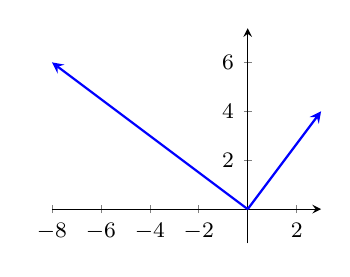
\begin{tikzpicture} 
\begin{axis}[axis equal, axis lines=middle,footnotesize]
    \addplot[quiver={u=3,v=4},blue,-stealth,thick] coordinates {(0,0)};
    \addplot[quiver={u=-8,v=6},blue,-stealth,thick] coordinates {(0,0)};
\end{axis}
\end{tikzpicture}}%
is an \idx{orthogonal set} as the two vectors have dot product\({}=3\cdot(-8)+4\cdot6=-24+24=0\)\,.
\end{example}


\begin{example} \label{eg:orthogtrio}
Let vectors \(\qv_1=(1,-2,2)\), \(\qv_2=(2,2,1)\) and \(\qv_3=(-2,1,2)\), illustrated in stereo below. 
Is \(\{\qv_1,\qv_2,\qv_3\}\) an \idx{orthogonal set}?
\begin{center}\qview{46}{50}{
\begin{tikzpicture} 
\begin{axis}[axis equal,footnotesize,font=\footnotesize
  ,view={\q}{30}]
\threev{1}{-2}{2}{\qv_1}
\threev[above]{2}{2}{1}{\qv_2}
\threev[left]{-2}{1}{2}{\qv_3}
\end{axis}
\end{tikzpicture}}
\end{center}

\begin{solution} 
Yes, because all the pairwise dot products are zero: \(\qv_1\cdot\qv_2=2-4+2=0\)\,; \(\qv_1\cdot\qv_3=-2-2+4=0\)\,; \(\qv_2\cdot\qv_3=-4+2+2=0\)\,. 
\end{solution}
\end{example}

\begin{definition} \label{def:orthoset} 
A set of non-zero vectors \(\{\hlist\qv k\}\) in~\(\RR^n\) is called an \bfidx{orthogonal set} if all pairs of distinct vectors in the set are \idx{orthogonal}: that is, \(\qv_i\cdot\qv_j=0\) whenever \(i\neq j\) for \(i,j=1,2,\ldots,k\)\,.
A set of vectors in~\(\RR^n\) is called an \bfidx{orthonormal set} if it is an \idx{orthogonal set} of \idx{unit vector}s.
\end{definition}

A single non-zero vector always forms an orthogonal set.  
A single unit vector always forms an orthonormal set.


\begin{example} \label{eg:}
Any set, or subset, of \idx{standard unit vector}s in~\(\RR^n\) (\autoref{def:stuniv}) are an \idx{orthonormal set} as they are all at right-angles (orthogonal), and all of length one.
\end{example}

\begin{example} \label{eg:}
Let vectors \(\qv_1=(\frac13,-\frac23,\frac23)\), \(\qv_2=(\frac23,\frac23,\frac13)\), \(\qv_3=(-\frac23,\frac13,\frac23)\).  
Show the set \(\{\qv_1,\qv_2,\qv_3\}\) is an orthonormal set.
\begin{solution} 
These vectors are all~\(1/3\) of the vectors in \autoref{eg:orthogtrio} and so are orthogonal.
They all have length one:
\(|\qv_1|^2={\frac19+\frac49+\frac49}=1\)\,;
\(|\qv_2|^2={\frac49+\frac49+\frac19}=1\)\,;
\(|\qv_3|^2={\frac49+\frac19+\frac49}=1\)\,.
Hence \(\{\qv_1,\qv_2,\qv_3\}\) is an orthonormal set in~\(\RR^3\). 
\end{solution}
\end{example}



\begin{activity}
Which one of the following sets of vectors is \emph{not} an orthogonal set?
\actposs{\(\{(2,3),(4,-1)\}\)}
{\(\{(-2,3),(6,4)\}\)}
{\(\{(-5,4)\}\)}
{\(\{\iv,\kv\}\)}
%\begin{parts}
%\item \(\{(2,3),(4,-1)\}\)\actans
%\item \(\{(-5,4)\}\)
%\item \(\{(-2,3),(6,4)\}\)
%\item \(\{\iv,\kv\}\)
%\end{parts}
\end{activity}

\index{orthonormal set|)}
\index{orthogonal set|)}




\subsubsection{Orthogonal matrices}
\index{orthogonal matrix|(}

\begin{example} \label{eg:}
\autoref{eg:orthogduo} showed \(\{(3,4),(-8,6)\}\) is an orthogonal set.  
The vectors have lengths five and ten, respectively, so dividing each by their length means \(\{(\frac35,\frac45),(-\frac45,\frac35)\}\) is an \idx{orthonormal set}.
Form the matrix~\(Q\) with these two vectors as its columns:
\[Q%=\begin{bmatrix} \qv_1&\qv_2 \end{bmatrix}
=\begin{bmatrix} \frac35&-\frac45\\\frac45&\frac35 \end{bmatrix}.\]
Then consider
\begin{equation*}
\tr QQ=\begin{bmatrix} \frac35&\frac45\\-\frac45&\frac35 \end{bmatrix}
\begin{bmatrix} \frac35&-\frac45\\\frac45&\frac35 \end{bmatrix}
=\begin{bmatrix} \frac{9+16}{25}&\frac{-12+12}{25}\\
\frac{-12+12}{25}&\frac{16+9}{25} \end{bmatrix}
=\begin{bmatrix} 1&0\\0&1 \end{bmatrix}.
\end{equation*}
Similarly \(Q\tr Q=I_2\)\,.
Consequently, the transpose~\(\tr Q\) is here the inverse of~\(Q\) (\autoref{def:invertible}).  
The transpose being the inverse is no accident.

Also no accident is that multiplication by this~\(Q\) gives the rotation illustrated at the start of this section,~(\S\ref{sec:omr}).
\end{example}




\begin{comment}
Could change this definition to $Q$~is {invertible} and $Q^{-1}=\tr Q$.  Then prove equivalence.  Use this for now.
\end{comment}

\begin{definition}[orthogonal matrices] \label{def:orthog} 
A square \(n\times n\) matrix~\(Q\) is called an \bfidx{orthogonal matrix} if \(\tr QQ=I_n\)\,.
Because of its special properties (\autoref{thm:orthog}),
multiplication by an orthogonal matrix is called a \bfidx{rotation and/or reflection};  
\footnote{Although herein we term multiplication by an orthogonal matrix as a `rotation' it generally is not a single rotation about a single axis.  
Instead, generally the `rotation' characterised by any one orthogonal matrix may be composed of a sequence of several rotations about different axes---each axis with a different orientation.}
for brevity and depending upon the circumstances it may be called just a \bfidx{rotation} or just a \bfidx{reflection}.
\end{definition}




\begin{activity}
For which of the following values of~\(p\) is the matrix \(Q=\begin{bmatrix} \frac12&p\\-p&\frac12 \end{bmatrix}\) orthogonal?
\actposs{\(p=\sqrt3/2\)}{\(p=-1/2\)}{\(p=3/4\)}{some other value}
%\begin{parts}
%\item \(p=-1/2\)
%\item \(p=\sqrt3/2\)
%\item \(p=3/4\)
%\item some other
%\end{parts}
\end{activity}



\begin{example} \label{eg:3dorthog}
In the following equation, check that the matrix is orthogonal, and hence solve the equation \(Q\xv=\bv\):
\begin{equation*}
\begin{bmatrix} \frac13&-\frac23&\frac23
\\\frac23&\frac23&\frac13
\\-\frac23&\frac13&\frac23 \end{bmatrix}\xv
=\begin{bmatrix} 0\\2\\-1 \end{bmatrix}.
\end{equation*} 
The \idx{stereo pair} below illustrates the rotation of the unit cube under multiplication by the matrix~\(Q\): every point~\xv\ in the (blue) unit cube, is mapped to the point~\(Q\xv\) to form the (red)~result.
\begin{center}
\def\unithousesize{footnotesize,height=5.5cm}
\ThreeD{1/3}{-2/3}{2/3}{2/3}{2/3}{1/3}{-2/3}{1/3}{2/3}
\end{center}
\begin{solution} In \script\ (recall the single quote (prime) gives the transpose, \autoref{tbl:mtlbops}),
\begin{verbatim}
Q=[1,-2,2;2,2,1;-2,1,2]/3
Q'*Q
\end{verbatim}
Since the product~\(\tr QQ\) is~\(I_3\), the matrix is orthogonal.  
Multiplying by~\(\tr Q\) both sides of the equation \(Q\xv=\bv\) gives \(\tr QQ\xv=\tr Q\bv\)\,; that is, \(I_3\xv=\tr Q\bv\), equivalently, \(\xv=\tr Q\bv\)\,.
Here,
\begin{verbatim}
x=Q'*[0;2;-1]
\end{verbatim}
\setbox\ajrqrbox\hbox{\qrcode{% check and solve orthog system
Q=[1,-2,2;2,2,1;-2,1,2]/3
Q'*Q
x=Q'*[0;2;-1]
}}%
\marginpar{\usebox{\ajrqrbox}}%
gives the solution \(\xv=(2,1,0)\).
\end{solution}
\end{example}


\begin{example} \label{eg:}
Given the matrix is orthogonal, solve the linear equation
\begin{equation*}
\begin{bmatrix} 
  \frac12&\frac12&\frac12&\frac12
\\\frac12&-\frac12&\frac12&-\frac12
\\\frac12&-\frac12&-\frac12&\frac12
\\\frac12&\frac12&-\frac12&-\frac12 \end{bmatrix}\xv
=\begin{bmatrix} 1\\-1\\1\\3 \end{bmatrix}.
\end{equation*}
\begin{solution} 
Denote the matrix by~\(Q\).
Given the matrix~\(Q\) is orthogonal, we know \(\tr QQ=I_4\). 
Just multiply the equation \(Q\xv=\bv\) by the transpose~\(\tr Q\) to deduce \(\tr QQ\xv=\tr Q\bv\), that is, \(\xv=\tr Q\bv\)\,.  
Here this equation gives the solution to be
\begin{equation*}
\xv=\begin{bmatrix} 
  \frac12&\frac12&\frac12&\frac12
\\\frac12&-\frac12&-\frac12&\frac12
\\\frac12&\frac12&-\frac12&-\frac12
\\\frac12&-\frac12&\frac12&-\frac12 \end{bmatrix}
\begin{bmatrix} 1\\-1\\1\\3 \end{bmatrix}
=\begin{bmatrix} 2\\2\\-2\\0 \end{bmatrix}.
\end{equation*}
\end{solution}
\end{example}


\begin{example} \label{eg:introt}
The marginal graph shows a rotation of the unit square. 
\def\unithousesize{footnotesize,grid} 
\marginpar{\TwoD{0.513}{0.857}{-0.858}{0.513}}%
From the graph estimate roughly the matrix~\(Q\) such that multiplication by~\(Q\) performs the rotation. 
Confirm that your estimated matrix is orthogonal (approximately).
\begin{solution} 
Consider what happens to the standard unit vectors:  multiplying~\(Q\) by~\((1,0)\) gives~\((0.5,-0.9)\) roughly (to one decimal place); whereas multiplying~\(Q\) by~\((0,1)\) gives~\((0.9,0.5)\) roughly.
To do this the matrix~\(Q\) must have these two vectors as its two columns, that is,
\begin{equation*}
Q\approx\begin{bmatrix} 0.5&0.9\\-0.9&0.5 \end{bmatrix}.
\end{equation*}
Let's check what happens to the corner point~\((1,1)\): \(Q(1,1)\approx (1.4,-0.4)\) which looks approximately correct.
To confirm orthogonality of~\(Q\), find
\begin{equation*}
\tr QQ=\begin{bmatrix} 0.5&-0.9\\0.9&0.5 \end{bmatrix}
\begin{bmatrix} 0.5&0.9\\-0.9&0.5 \end{bmatrix}
=\begin{bmatrix} 1.06&0\\0&1.06 \end{bmatrix}\approx I_2\,,
\end{equation*}
and so \(Q\)~is approximately orthogonal.
\end{solution}
\end{example}


Because orthogonal matrices represent rotations, they arise frequently in engineering and scientific mechanics of bodies.
Also, the ease in solving equations with orthogonal matrices puts orthogonal matrices at the heart of coding and decoding photographs (jpeg), videos (mpeg), signals (Fourier transforms), and so on.
Furthermore, an extension of orthogonal matrices to complex valued matrices, the so-called unitary matrices, is at the core of quantum physics and quantum computing.
Moreover, the next \autoref{sec:fisvd} establishes that orthogonal matrices express the orientation of the action of \emph{every} matrix and hence are a vital component of solving linear equations in general.
But to utilise orthogonal matrices across the wide range of applications we need to establish the following properties.




\begin{theorem} \label{thm:orthog}
For every \idx{square matrix}~\(Q\),  the following statements are equivalent:
\begin{enumerate}
\item\label{thm:orthog:0} \(Q\)~is an \idx{orthogonal matrix};
\item\label{thm:orthog:ii} the \idx{column vector}s of~\(Q\) form an \idx{orthonormal set}; 
\item\label{thm:orthog:i} \(Q\)~is \idx{invertible} and \(Q^{-1}=\tr Q\);
\item\label{thm:orthog:ia} \(\tr Q\) is an \idx{orthogonal matrix};
\item\label{thm:orthog:iii} the \idx{row vector}s of~\(Q\) form an \idx{orthonormal set};
\item\label{thm:orthog:iv} multiplication by~\(Q\) preserves all lengths and angles (and hence corresponds to our intuition of a \idx{rotation and/or reflection}).
%\item\label{thm:orthog:v}  
%if \(Q_1\) and~\(Q_2\) are orthogonal matrices of the same size, then so is the product~\(Q_1Q_2\).
\end{enumerate}
\end{theorem}

\begin{proof} 
Write \(n\times n\) matrix \(Q=\begin{bmatrix} \qv_1&\qv_2&\cdots&\qv_n \end{bmatrix}\) in terms of its \(n\)~columns \hlist\qv n.
So then the transpose~\(\tr Q\) has the vectors \hlist\qv n\ as its rows---the \(i\)th~row being the row vector~\(\tr\qv_i\).
\begin{description}
\item[\ref{thm:orthog:0}$\iff$\ref{thm:orthog:ii}]   Consider
\begin{eqnarray*}
\tr QQ
&=&\begin{bmatrix} \tr\qv_1\\\tr\qv_2\\\vdots\\\tr\qv_n \end{bmatrix}
\begin{bmatrix} \qv_1&\qv_2&\cdots&\qv_n \end{bmatrix}
\\&=&\begin{bmatrix} \tr\qv_1\qv_1&\tr\qv_1\qv_2&\cdots&\tr\qv_1\qv_n 
\\ \tr\qv_2\qv_1&\tr\qv_2\qv_2&\cdots&\tr\qv_2\qv_n 
\\\vdots&\vdots&\ddots&\vdots
\\ \tr\qv_n\qv_1&\tr\qv_n\qv_2&\cdots&\tr\qv_n\qv_n \end{bmatrix}
\\&=&\begin{bmatrix} \qv_1\cdot\qv_1&\qv_1\cdot\qv_2&\cdots&\qv_1\cdot\qv_n 
\\ \qv_2\cdot\qv_1&\qv_2\cdot\qv_2&\cdots&\qv_2\cdot\qv_n 
\\\vdots&\vdots&\ddots&\vdots
\\ \qv_n\cdot\qv_1&\qv_n\cdot\qv_2&\cdots&\qv_n\cdot\qv_n \end{bmatrix}
\end{eqnarray*}
Matrix~\(Q\) is orthogonal if and only if this product is the identity  (\autoref{def:orthog}) which is if and only if \(\qv_i\cdot\qv_j=0\) for \(i\neq j\) and \(|\qv_i|^2=\qv_i\cdot\qv_i=1\), that is, if and only if the columns~\(\qv_i\) are orthonormal (\autoref{def:orthoset}).

\item[\ref{thm:orthog:ii}$\implies$\ref{thm:orthog:i}] 
First, consider the homogeneous system \(\tr Q\xv=\ov\) for \(\xv\) in~\(\RR^n\).
We establish \(\xv=\ov\) is the only solution.
The system \(\tr Q\xv=\ov\), written in terms of the orthonormal columns of~\(Q\), is 
\begin{equation*}
\begin{bmatrix} \tr\qv_1\\\tr\qv_2\\\vdots\\\tr\qv_n \end{bmatrix}\xv
=\begin{bmatrix} \tr\qv_1\xv\\\tr\qv_2\xv\\\vdots\\\tr\qv_n\xv \end{bmatrix}
=\begin{bmatrix} \qv_1\cdot\xv\\\qv_2\cdot\xv\\\vdots\\\qv_n\cdot\xv \end{bmatrix}
=\begin{bmatrix} 0\\0\\\vdots\\0 \end{bmatrix}.
\end{equation*}
Since the dot products are all zero, either \(\xv=\ov\) or \(\xv\)~is orthogonal (at right angles) to all of the \(n\)~orthonormal vectors~\(\{\hlist\qv n\}\).
In~\(\RR^n\) we cannot have \((n+1)\) non-zero vectors all at right angles to each other (\autoref{thm:orthcomp}), consequently \(\xv=\ov\) is the only possibility as the solution of \(\tr Q\xv=\ov\)\,.
% this argument is by completeness of the columns of Q in RR^n

%\begin{aside}
%Incidentally,  this matrix~\(X\) would the projection onto the (here empty) complement of \(\Span Q\).
%\end{aside}
Second, let \(n\times n\) matrix \(X=I_n-Q\tr Q\).
Pre-multiply by~\(\tr Q\): \(\tr QX
=\tr Q(I_n-Q\tr Q)
=\tr QI_n-(\tr QQ)\tr Q
=\tr QI_n-I_n\tr Q
=\tr Q-\tr Q
=O_n\)\,.
That is, \(\tr QX=O_n\)\,. 
But each column of \(\tr QX=O_n\) is of the form \(\tr Q\xv=\ov\) which we know requires \(\xv=\ov\)\,, hence \(X=O_n\)\,.
Then \(X=I_n-Q\tr Q=O_n\) which rearranged gives \(Q\tr Q=I_n\)\,. 
Put \(Q\tr Q=I_n\) together with \(\tr QQ=I_n\) (\autoref{def:orthog}),  then by \autoref{def:invertible}  \(Q\)~is invertible with inverse~\(\tr Q\).

\item[\ref{thm:orthog:i}$\implies$\ref{thm:orthog:0},\ref{thm:orthog:ia}]
Part~\ref{thm:orthog:i} asserts \(Q\)~is invertible with inverse~\(\tr Q\): by \autoref{def:invertible} of the inverse, \(\tr QQ=Q\tr Q=I_n\).  
Since \(\tr QQ=I_n\)\,, matrix~\(Q\) is orthogonal.
 
Since \(I_n=Q\tr Q=\tr{(\tr Q)}\tr Q\), by \autoref{def:orthog} \(\tr Q\)~is orthogonal.

\item[\ref{thm:orthog:ia}$\iff$\ref{thm:orthog:iii}] 
The proof is similar to that for \ref{thm:orthog:0}$\iff$\ref{thm:orthog:ii}, but for the rows of~\(Q\) and \(Q\tr Q=I_n\)\,.

\item[\ref{thm:orthog:iii}$\implies$\ref{thm:orthog:i}] 
Similar to that for \ref{thm:orthog:ii}$\implies$\ref{thm:orthog:i}, but for the rows of~\(Q\), \(Q\xv=\ov\) and \(X=I_n-\tr QQ\)\,.

\item[\ref{thm:orthog:0}$\implies$\ref{thm:orthog:iv}] 
We prove that multiplication by orthogonal~\(Q\) preserves all lengths and angles, as illustrated in Examples~\ref{eg:3dorthog} and~\ref{eg:introt}, by comparing the properties of transformed vectors~\(Q\uv\) with the properties of the original~\uv.
For any vectors~\(\uv,\vv\) in~\(\RR^n\), consider the dot product
\((Q\uv)\cdot(Q\vv)=\tr{(Q\uv)}Q\vv
=\tr\uv\tr QQ\vv
=\tr\uv I_n\vv
=\tr\uv\vv=\uv\cdot\vv\)\,.  
Now let's use this identity that \((Q\uv)\cdot(Q\vv)=\uv\cdot\vv\)\,.
\begin{itemize}
\item Firstly, the length \(|Q\uv|=\sqrt{(Q\uv)\cdot(Q\uv)}=\sqrt{\uv\cdot\uv}=|\uv|\) is preserved, and correspondingly for~\vv.
\item Secondly, let \(\theta\)~be the angle between \uv\ and~\vv\ and \(\theta'\)~be the angle between \(Q\uv\) and~\(Q\vv\) (recall \(0\leq\text{angle}\leq\pi\)), then
\begin{equation*}
\cos\theta'=\frac{(Q\uv)\cdot(Q\vv)}{|Q\uv||Q\vv|}
=\frac{\uv\cdot \vv}{|\uv||\vv|}
=\cos\theta\,.
\end{equation*}
Since \(\cos\theta'=\cos\theta\) and the cosine is 1-1 for \(0\leq\text{angles}\leq\pi\)\,, all angles are preserved.
\end{itemize}

\item[\ref{thm:orthog:iv}$\implies$\ref{thm:orthog:ii}]
Look at the consequences of matrix~\(Q\) preserving all lengths and angles when applied to the standard unit vectors \hlist\ev n.
Observe \(Q\ev_j=\qv_j\)\,, the \(j\)th~column of matrix~\(Q\).
Then for all~\(j\), the length of the \(j\)th~column \(|\qv_j|=|Q\ev_j|=|\ev_j|=1\) by the preservation of the length of the standard unit vector.
Also, for all~\(i\neq j\) the dot product of columns \(\qv_i\cdot\qv_j=|\qv_i||\qv_j|\cos\theta'=1\cdot1\cdot\cos\frac\pi2=0\) where \(\theta'\)~is the angle between \(\qv_i\) and~\(\qv_j\) which is the angle between \(\ev_i\) and~\(\ev_j\) by preservation, namely the angle~\(\frac\pi2\).
That is, the columns of~\(Q\) form an orthonormal set. 

%\item[\ref{thm:orthog:v}]  Exercise: consider \(\tr{(Q_1Q_2)}Q_1Q_2\).
\end{description}
\end{proof}


Another important property,  proved by \autoref{ex:orthoprod}, is that the product of orthogonal matrices is also an orthogonal matrix.

\begin{example} \label{eg:}
Show that these matrices are orthogonal and hence write down their inverses:
\begin{equation*}
\begin{bmatrix} 0&0&1\\1&0&0\\0&1&0 \end{bmatrix},\quad
\begin{bmatrix} \cos\theta&-\sin\theta\\\sin\theta&\cos\theta \end{bmatrix}.
\end{equation*}

\begin{solution} 
For the first matrix, by inspection each column is a unit vector, and each column is orthogonal to each other: since the matrix has orthonormal columns, then the matrix is orthogonal (\autoref{thm:orthog:ii}).
Its inverse is the transpose (\autoref{thm:orthog:i})
\begin{equation*}
\begin{bmatrix} 0&1&0\\0&0&1\\1&0&0 \end{bmatrix}.
\end{equation*}

For the second matrix the two columns are unit vectors as
\(|(\cos\theta,\sin\theta)|^2=\cos^2\theta+\sin^2\theta=1\) and \(|(-\sin\theta,\cos\theta)|^2=\sin^2\theta+\cos^2\theta=1\)\,.
The two columns are orthogonal as the dot product \((\cos\theta,\sin\theta)\cdot(-\sin\theta,\cos\theta)=-\cos\theta\,\sin\theta+\sin\theta\,\cos\theta=0\)\,.  
Since the matrix has orthonormal columns, then the matrix is orthogonal (\autoref{thm:orthog:ii}).
Its inverse is the transpose (\autoref{thm:orthog:i})
\begin{equation*}
\begin{bmatrix} \cos\theta&\sin\theta\\-\sin\theta&\cos\theta \end{bmatrix}.
\end{equation*}
\end{solution}
\end{example}




\begin{example} \label{eg:}
The following graphs illustrate the transformation of the unit square through multiplying by some different matrices. 
Using \autoref{thm:orthog:iv}, which transformations appear to be that of multiplying by an orthogonal matrix?
% a=randn(2),svd(a)',[b,r]=qr(a),det(b)
\begin{parts}
\item \TwoD{-1.15}{2.44}{0.95}{0.82}
\item \TwoD{0.64}{-0.77}{0.77}{0.64}
\item \TwoD{-0.84}{0.54}{0.54}{0.84}
\item \TwoD{1.33}{-0.52}{0.82}{0.35}
\end{parts}

\begin{solution} \ 
\begin{parts}
\item No---the square is stretched and angles changed.
\item Yes---the square is just rotated.
\item Yes---the square is rotated and reflected.
\item No---the square is squashed and angles changed.
\end{parts}
\end{solution}
\end{example}




\begin{activity}
The following graphs illustrate the transformation of the unit square through multiplying by some different matrices. 
\begin{itemize}
\item Which transformation appears to be that of multiplying by an orthogonal matrix?
\actposs{\TwoD{-0.85}{-0.52}{-0.52}{0.85}}
{\TwoD{-1.67}{1.54}{1.07}{2.11}}
{\TwoD{-1.3}{0}{0}{0.8}}
{\TwoD{1.06}{-1.02}{-0.16}{-0.51}}
%\begin{parts}
%\item \TwoD{-1.67}{1.54}{1.07}{2.11}
%\item \TwoD{-1.3}{0}{0}{0.8}
%\item \TwoD{-0.85}{-0.52}{-0.52}{0.85}
%\item \TwoD{1.06}{-1.02}{-0.16}{-0.51}
%\end{parts}
\item Further, which of the above transformations appear to be that of multiplying by a diagonal matrix?
\end{itemize}
\end{activity}





\begin{example} \label{eg:}
The following \idx{stereo pair}s illustrate the transformation of the unit cube through multiplying by some different matrices: using \autoref{thm:orthog:iv}, which transformations appear to be that of multiplying by an orthogonal matrix?
% a=randn(3),svd(a)',[b,r]=qr(a),det(b)
\begin{enumerate}
\item \ThreeD{-0.73}{-0.64}{-0.24
}{0.68}{-0.73}{-0.11
}{-0.10}{-0.25}{0.96}

\item \ThreeD{-1.26}{-0.56}{-1.01
}{1.17}{-1.58}{-0.91
}{-0.18}{-0.33}{1.35}

\def\unithousesize{small}
\item \ThreeD{-0.05}{1.50}{-0.51
}{-2.35}{0.49}{0.35
}{-0.76}{0.28}{-0.18}

%\item \ThreeD{0.02}{1.00}{-0.08
%}{0.95}{-0.04}{-0.31
%}{0.31}{0.07}{0.95}
%
%\item \ThreeD{0.83}{0.10}{-1.61
%}{0.21}{0.41}{-0.41
%}{-0.17}{-0.69}{-0.15}
%
%\item \ThreeD{0.95}{0.29}{-0.12
%}{0.24}{-0.44}{0.86
%}{-0.19}{0.85}{0.49}

\def\unithousesize{small}
\item \ThreeD{0.02}{0.20}{0.98
}{0.99}{-0.16}{0.01
}{-0.16}{-0.97}{0.20}
\end{enumerate}

\begin{solution} 
\begin{enumerate}
\item Yes---the cube is just rotated.
\item No---the cube is stretched and angles changed.
\item No---the cube is stretched and angles changed.
\item Yes---the cube is just rotated and reflected.
\end{enumerate}
\end{solution}
\end{example}



%\begin{comment}
%Some more examples of these properties??
%\end{comment}

\index{orthogonal matrix|)}





\begin{comment}
Could have a section on GF(2): that is, inverses of 0-1 matrices mod 2??  Relevant to computer science encoding and encryption---somehow.  Matlab/octave supports modular computation via gf() something and some package, respectively.
\end{comment}





\subsection{Exercises}


\begin{exercise} \label{ex:abinv} 
By direct multiplication, both ways, confirm that for each of the following pairs, matrix~\(B\) is an inverse of matrix~\(A\), or not.
\begin{enumerate}
% a=round(randn(4)*3)+0, b=inv(a)+0
\item \(A=\begin{bmatrix} 0&-4
\\4&4 \end{bmatrix}\), 
\(B=\begin{bmatrix} 1/4&1/4
\\-1/4&0 \end{bmatrix}\)
\answer{Inverse.}

\item \(A=\begin{bmatrix} -3&3
\\-3&1 \end{bmatrix}\), 
\(B=\begin{bmatrix} 1/6&-1/2
\\1/2&-1/2 \end{bmatrix}\)
\answer{Inverse.}

\item \(A=\begin{bmatrix} 5&-1
\\3&-2 \end{bmatrix}\), 
\(B=\begin{bmatrix} 3/7&-1/7
\\3/7&-5/7 \end{bmatrix}\)
\answer{Not inverse.}

\item \(A=\begin{bmatrix} -1&1
\\-5&-1 \end{bmatrix}\), 
\(B=\begin{bmatrix} -1/6&-1/6
\\5/6&-1/6 \end{bmatrix}\)
\answer{Inverse.}

\item \(A=\begin{bmatrix} -2&4&2
\\1&1&-1
\\1&-1&1 \end{bmatrix}\), 
\(B=\begin{bmatrix} 0&1/2&1/2
\\1/6&1/3&0
\\1/6&-1/6&1/2 \end{bmatrix}\)
\answer{Inverse.}

\item \(A=\begin{bmatrix} -3&0&-1
\\1&4&2
\\3&-4&-1 \end{bmatrix}\), 
\(B=\begin{bmatrix} 1&1&1
\\7/4&3/2&5/4
\\-4&-3&-3 \end{bmatrix}\)
\answer{Inverse.}

\item \(A=\begin{bmatrix} -3&-3&3
\\4&3&-3
\\-2&-1&4 \end{bmatrix}\), 
\(B=\begin{bmatrix} 1&1&0
\\-1&-2/3&1/3
\\2/9&1/3&1/3 \end{bmatrix}\)
\answer{Not inverse.}

%for j=1:99, a=round(randn(4)*3)+0; if abs(det(a))<10,break,end,end,a=a,b=inv(a)+0

\item \(A=\begin{bmatrix} -1&3&4&-1
\\2&2&-2&0
\\1&2&-2&0
\\4&2&4&-1 \end{bmatrix}\), 
\setbox\ajrqrbox\hbox{\qrcode{% inverses?
A=[-1 3 4 -1
 2 2 -2 0
 1 2 -2 0
 4 2 4 -1 ]
B=[0 1 -1 0
 1 5 -5 -1
 1 11/2 -6 -1
 6 36 -38 -7 ]
}}%
\marginpar{\usebox{\ajrqrbox}}%
\(B=\begin{bmatrix} 0&1&-1&0
\\1&5&-5&-1
\\1&11/2&-6&-1
\\6&36&-38&-7 \end{bmatrix}\), use \script
\answer{Inverse.}

\item \(A=\begin{bmatrix} 0&-2&-2&-3
\\-4&-5&0&1
\\-2&0&4&5
\\-1&1&0&-2 \end{bmatrix}\), 
\setbox\ajrqrbox\hbox{\qrcode{% inverses?
A=[0 -2 -2 -3
 -4 -5 0 1
 -2 0 4 5
 -1 1 0 -2 ]
B=[2/3 -1/3 1/3 -1/3
 -2/3 1/9 -1/3 2/9
 7/6 -4/9 5/6 1/9
 -2/3 2/9 -1/3 -2/9 ]
}}%
\marginpar{\usebox{\ajrqrbox}}%
\(B=\begin{bmatrix} 2/3&-1/3&1/3&-1/3
\\-2/3&1/9&-1/3&2/9
\\7/6&-4/9&5/6&1/9
\\-2/3&2/9&-1/3&-2/9 \end{bmatrix}\), use \script
\answer{Inverse.}

\item \(A=\begin{bmatrix} 0&0&7&-1
\\2&4&0&4
\\-2&-2&1&-2
\\-3&-3&1&-3 \end{bmatrix}\), 
\setbox\ajrqrbox\hbox{\qrcode{% inverses?
A=[0 0 7 -1
 2 4 0 4
 -2 -2 1 -2
 -3 -3 1 -3 ]
B=[0 -1/2 2 -2
 1 1/2 -21 15
 0 0 3 -2
 -1 0 21 -14 ]
}}%
\marginpar{\usebox{\ajrqrbox}}%
\(B=\begin{bmatrix} 0&-1/2&2&-2
\\1&1/2&-21&15
\\0&0&3&-2
\\-1&0&21&-14 \end{bmatrix}\), use \script
\answer{Not inverse.}

\item \(A=\begin{bmatrix} 1&-7&-4&3
\\0&2&1&-1
\\0&-2&-3&2
\\3&-2&-4&1 \end{bmatrix}\), 
\setbox\ajrqrbox\hbox{\qrcode{% inverses?
A=[1 -7 -4 3
 0 2 1 -1
 0 -2 -3 2
 3 -2 -4 1 ]
B=[-2 -7 -1 1
 -1 -8/3 0 1/3
 -2 -22/3 -1 2/3
 -4 -41/3 -1 4/3 ]
}}%
\marginpar{\usebox{\ajrqrbox}}%
\(B=\begin{bmatrix} -2&-7&-1&1
\\-1&-8/3&0&1/3
\\-2&-22/3&-1&2/3
\\-4&-41/3&-1&4/3 \end{bmatrix}\), use \script
\answer{Inverse.}

\end{enumerate}
\end{exercise}




\begin{exercise} \label{ex:2x2det} 
Use the direct formula of \autoref{thm:2x2det} to calculate the inverse, when it exists, of the following \(2\times2\) matrices.
% a=round(randn(2)*3)+0, b=inv(a)+0
\begin{parts}
\item \(\begin{bmatrix} -2&2
\\-1&4 \end{bmatrix}\)
\answer{\(\begin{bmatrix} -2/3&1/3
\\-1/6&1/3 \end{bmatrix}\)}

\item \(\begin{bmatrix} -5&-10
\\-1&-2 \end{bmatrix}\)
\answer{No inverse.}

\item \(\begin{bmatrix} -2&-4
\\5&2 \end{bmatrix}\)
\answer{\(\begin{bmatrix} 1/8&1/4
\\-5/16&-1/8 \end{bmatrix}\)}

\item \(\begin{bmatrix} -3&2
\\-1&-2 \end{bmatrix}\)
\answer{\(\begin{bmatrix} -1/4&-1/4
\\1/8&-3/8 \end{bmatrix}\)}

\item \(\begin{bmatrix} 2&-4
\\3&0 \end{bmatrix}\)
\answer{\(\begin{bmatrix} 0&1/3
\\-1/4&1/6 \end{bmatrix}\)}

\item \(\begin{bmatrix} -0.6&-0.9
\\0.8&-1.4 \end{bmatrix}\)
\answer{\(\begin{bmatrix} -0.8974&0.5769
\\-0.5128&-0.3846 \end{bmatrix}\)}

\item \(\begin{bmatrix} 0.3&0
\\0.9&1.9 \end{bmatrix}\)
\answer{\(\begin{bmatrix} 3.3333&0
\\-1.5789&0.5263 \end{bmatrix}\)}

\item \(\begin{bmatrix} 0.6&0.5
\\-0.3&0.5 \end{bmatrix}\)
\answer{\(\begin{bmatrix} 10/9&-10/9
\\2/3&4/3 \end{bmatrix}\)}

\end{parts}
\end{exercise}




\begin{exercise} \label{ex:} 
Given the inverses of Exercises~\ref{ex:abinv}, solve each of the following systems of linear equations with a matrix-vector multiply (\autoref{thm:invuniqsol}).
\begin{parts}
\item \(\begin{cases} -4y=1\\4x+4y=-5 \end{cases}\)
\answer{\((x,y)=(-1,-1/4)\)}

\item \(\begin{cases} -3p+3q=3\\-3p+q=-1 \end{cases}\)
\answer{\((p,q)=(1,2)\)}

\item \(\begin{cases} m-x=1\\-m-5x=-1 \end{cases}\)
\answer{\(x=0,\ m=1\)}

\item \(\begin{cases} -3x-z=3\\ x+4y+2z=-3\\ 3x-4y-z=2 \end{cases}\)
\answer{\((x,y,z)=(2,13/4,-9)\)}

\item \(\begin{cases} 2p-2q+4r=-1\\ -p+q+r=-2\\ p+q-r=1 \end{cases}\)
\answer{\((q,r,p)=(-1/2,-5/6,2/3)\)}

\item \(\begin{cases} -x_1+3x_2+4x_3-x_4=0
\\2x_1+2x_2-2x_3=-1
\\x_1+2x_2-2x_3=3
\\4x_1+2x_2+4x_3-x_4=-5 \end{cases}\)
\answer{\(\xv=(-1,1,1,4)\)}

\item \(\begin{cases} p-7q-4r+3s=-1
\\2q+r-s=-5
\\-2q-3r+2s=3
\\3p-2q-4r+s=-1 \end{cases}\)
\answer{\((p,q,r,s)=(33,14,35,68)\)}

\item \(\begin{cases}-3b-2c-2d=4
\\-4a+b-5d=-3
\\-2a+5b+4c=-2
\\-a-2b+d=0 \end{cases}\)
\answer{\((a,d,c,b)=(3,-7/3,13/3,-8/3)\)}

\end{parts}
\end{exercise}




\begin{exercise} \label{ex:} 
Given the following information about solutions of systems of linear equations, write down if the matrix associated with each system is invertible, or not, or there is not enough given information to decide.  
Give reasons.
\begin{enumerate}
\item The general solution is \((-2,1,2,0,2)\).
\answer{Invertible}

\item A solution of a system is \((2.4,-2.8,-3.6,-2.2,-3.8)\).
\answer{Not enough information}

\item A solution of a homogeneous system is \((0.8,0.4,-2.3,2.5)\).
\answer{Not invertible.}

\item The general solution of a system is \((4,1,0,2)t\) for all~\(t\).
\answer{Not invertible.}

\item The general solution of a homogeneous system is \((0,0,0,0)\).
\answer{Invertible.}

\item A solution of a homogeneous system is \((0,0,0,0,0)\).
\answer{Not enough information.}

\end{enumerate}
\end{exercise}





\begin{exercise} \label{ex:} 
Use \script\ to generate some random matrices of a suitable size of your choice, and some random scalar exponents (see \autoref{tbl:mtlbops}).
Then confirm the properties of \index{inverse matrix}inverse matrices given by \autoref{thm:pasm}.
For the purposes of this exercise, use the \script\ function \index{inv()@\texttt{inv()}}\verb|inv(A)| that computes the inverse of the matrix~\(A\) if it exists (as commented, remember that computing the inverse of a matrix is generally inappropriate---the inverse is primarily a  theoretical device---this exercise only computes the inverse for educational purposes).
Record all your commands and the output from \script.
\end{exercise}







\begin{exercise} \label{ex:} 
Consider \autoref{thm:invprop} on the properties of the inverse. Invoking properties of matrix operations from \autoref{sec:fapmo},
\begin{enumerate}
\item prove Part~\ref{thm:invpropb} using associativity, and
\item prove Part~\ref{thm:invpropd} using the transpose.
\end{enumerate}
\end{exercise}



\begin{exercise} \label{ex:} 
Recall the properties of the inverse, \autoref{thm:invprop}, and matrix operations, \autoref{sec:fapmo}.
\begin{aside}
This is the \idx{Woodbury generalisation} of the \idx{Sherman--Morrison formula}.  It is used to update matrices while searching for optima and solutions.
\end{aside}%
Use these properties to prove that for every \(n\times n\) invertible matrix~\(A\), and every \(n\times m\) matrices~\(U\) and~\(V\) such that \(I_m+\tr VA^{-1}U\) is invertible, then the matrix \(A+U\tr V\) is invertible and
\begin{equation*}
(A+U\tr V)^{-1}=A^{-1}-(A^{-1}U)(I_m+\tr VA^{-1}U)^{-1}(\tr VA^{-1}).
\end{equation*}
Hint: directly check \autoref{def:invertible}.
\end{exercise}





\begin{exercise} \label{ex:} 
Using the inverses identified in \autoref{ex:abinv}, and matrix multiplication, calculate the following matrix powers.
\begin{parts}
\item \(\begin{bmatrix} 0&-4\\4&4 \end{bmatrix}^{-2}\)
\answer{\(\begin{bmatrix} 0&1/16
\\-1/16&-1/16 \end{bmatrix}\)}

\item \(\begin{bmatrix} 0&-4\\4&4 \end{bmatrix}^{-3}\)
\answer{\(\begin{bmatrix} -1/64&0
\\0&-1/64 \end{bmatrix}\)}

\item \(\begin{bmatrix} -3&3
\\-3&1 \end{bmatrix}^{-2}\)
\answer{\(\begin{bmatrix} -2/9&1/6
\\-1/6&0 \end{bmatrix}\)}

\item \(\begin{bmatrix} -1/6&-1/6
\\5/6&-1/6 \end{bmatrix}^{-4}\)
\answer{\(\begin{bmatrix} -4&16
\\-80&-4 \end{bmatrix}\)}

\item \(\begin{bmatrix} -3&0&-1
\\1&4&2
\\3&-4&-1 \end{bmatrix}^2\)
\answer{\(\begin{bmatrix} -5/4&-1/2&-3/4
\\-5/8&1/4&-1/8
\\11/4&1/2&5/4 \end{bmatrix}\)}

\item \(\begin{bmatrix} 0&1/2&1/2
\\1/6&1/3&0
\\1/6&-1/6&1/2 \end{bmatrix}^{-2}\)
\answer{\(\begin{bmatrix} 10&-6&-6
\\-2&6&0
\\-2&2&4 \end{bmatrix}\)}

\item \(\begin{bmatrix} -1&3&4&-1
\\2&2&-2&0
\\1&2&-2&0
\\4&2&4&-1 \end{bmatrix}^{-2}\) use \script
\answer{\(\begin{bmatrix} 0&-1/2&1&0
\\-6&-75/2&42&7
\\-13/2&-81/2&91/2&15/2
\\-44&-275&308&51 \end{bmatrix}\)}

\item \(\begin{bmatrix} -2&-7&-1&1
\\-1&-8/3&0&1/3
\\-2&-22/3&-1&2/3
\\-4&-41/3&-1&4/3 \end{bmatrix}^{-3}\) use \script.
\answer{\(\begin{bmatrix} 25&-96&-46&32
\\-6&25&11&-8
\\0&-40&-15&16
\\18&-76&-41&29 \end{bmatrix}\)}

\end{parts}
\end{exercise}




\begin{exercise} \label{ex:} 
Which of the following matrices are \index{diagonal matrix}diagonal? 
For those that are diagonal, write down how they may be represented with the \(\diag\) function (algebraic, not \script).
% m=1+ceil(4*rand);n=1+ceil(4*rand); a=round((diag(randn(ceil(min(m,n)*sqrt(rand)),1),m,n)+full(sprandn(m,n,-log(rand)/m/n*2)))*3)+0

\begin{parts}
\item \(\begin{bmatrix} 9&0&0
\\0&-5&0
\\0&0&4 \end{bmatrix}\)
\answer{\(\diag(9,-5,4)\)}

\item \(\begin{bmatrix} 0&0&1
\\0&2&0
\\-2&0&0 \end{bmatrix}\)
\answer{Not diagonal.}

\item \(\begin{bmatrix} -5&0&0&0&0
\\0&1&0&0&0
\\0&0&9&0&0
\\0&0&0&1&0
\\0&0&0&0&0 \end{bmatrix}\)
\answer{\(\diag(-5,1,9,1,0)\)}

\item \(\begin{bmatrix} 6&0&0&0
\\0&1&0&-9
\\0&0&0&0
\\0&0&0&0 \end{bmatrix}\)
\answer{Not diagonal.}

\item \(\begin{bmatrix} 0&0&0
\\0&-1&0
\\0&0&-5
\\0&0&0
\\0&0&0 \end{bmatrix}\)
\answer{\(\diag_{5\times3}(0,-1,-5)\)}

\item \(\begin{bmatrix} 1&0
\\0&1
\\0&0
\\2&0
\\0&0 \end{bmatrix}\)
\answer{Not diagonal.}

\item \(\begin{bmatrix} 2&0&0
\\0&1&0
\\0&0&0 \end{bmatrix}\)
\answer{\(\diag(2,1,0)\)}

\item \(\begin{bmatrix} 0&0&0
\\0&2&0 \end{bmatrix}\)
\answer{\(\diag_{2\times3}(0,2)\)}

\item \(\begin{bmatrix} -3&0&c&0&0
\\0&2&0&0&0
\\0&0&-2&0&0
\\0&0&0&0&0 \end{bmatrix}\)
\answer{Diagonal only when \(c=0\).}

\item \(\begin{bmatrix} -3c&0&0&-4d
\\0&5b&0&0
\\a&0&0&0 \end{bmatrix}\)
\answer{Diagonal only when \(a=d=0\).}

\end{parts}
\end{exercise}




\begin{exercise} \label{ex:} 
Write down the individual algebraic equations represented by each of the following diagonal matrix-vector equations.
Hence, where possible solve each system.
%m=1+ceil(4*rand);n=1+ceil(4*rand); a=round(diag(randn(ceil(min(m,n)*sqrt(rand)),1),m,n)*3)+0,b=round(randn(m,1)*3)+0
\begin{enumerate}
\item \(\begin{bmatrix} -4&0&0&0&0
\\0&1&0&0&0
\\0&0&-2&0&0
\\0&0&0&1&0
\\0&0&0&0&-3 \end{bmatrix}
\begin{bmatrix}x_1\\x_2\\x_3\\x_4\\x_5\end{bmatrix}
=\begin{bmatrix} 6
\\-1
\\-4
\\-2
\\4 \end{bmatrix}\)
\answer{\(\xv=(-3/2,-1,2,-2,-4/3)\)}

\item \(\begin{bmatrix} 0&0&0&0
\\0&4&0&0
\\0&0&-1&0 \end{bmatrix}
\begin{bmatrix}x_1\\x_2\\x_3\\x_4\end{bmatrix}
=\begin{bmatrix} -8
\\3
\\-1 \end{bmatrix}\)
\answer{No solution.}

\item \(\begin{bmatrix} 4&0
\\0&0 \end{bmatrix}
\begin{bmatrix}x\\y\end{bmatrix}
=\begin{bmatrix} 5
\\0 \end{bmatrix}\)
\answer{\((x,y)=(5/4,t)\) for all~\(t\)}

\item \(\begin{bmatrix} -6&0&0&0&0
\\0&4&0&0&0
\\0&0&2&0&0 \end{bmatrix}
\begin{bmatrix}x_1\\x_2\\x_3\\x_4\\x_5\end{bmatrix}
=\begin{bmatrix} 0
\\-1
\\2 \end{bmatrix}\)
\answer{\(\xv=(0,-1/4,1,s,t)\) for all~\(s,t\)}

\item \(\begin{bmatrix} -3&0&0&0&0
\\0&-4&0&0&0
\\0&0&-6&0&0
\\0&0&0&0&0 \end{bmatrix}
\begin{bmatrix}x_1\\x_2\\x_3\\x_4\\x_5\end{bmatrix}
=\begin{bmatrix} -5
\\-5
\\1
\\-1 \end{bmatrix}\)
\answer{No solution.}

\item \(\begin{bmatrix} 0.5&0&0&0
\\0&0.2&0&0 \end{bmatrix}
\begin{bmatrix}w\\x\\y\\z\end{bmatrix}
=\begin{bmatrix} 3
\\-1 \end{bmatrix}\)
\answer{\((w,x,y,z)=(6,-5,s,t)\) for all~\(s,t\)}

\item \(\begin{bmatrix} 1&0&0&0
\\0&-3&0&0
\\0&0&-3&0
\\0&0&0&0 \end{bmatrix}
\begin{bmatrix}p\\q\\r\\s\end{bmatrix}
=\begin{bmatrix} -2
\\-6
\\8
\\0 \end{bmatrix}\)
\answer{\((p,q,r,s)=(-2,2,-8/3,t)\) for all~\(t\)}

\item \(\begin{bmatrix} -1&0&0&0
\\0&3&0&0
\\0&0&0&0 \end{bmatrix}
\begin{bmatrix}&\end{bmatrix}
=\begin{bmatrix} -3
\\0
\\3 \end{bmatrix}\)
\answer{No solution.}

\end{enumerate}
\end{exercise}





\begin{exercise} \label{ex:} 
In each of the following illustrations, the unit square (blue) is transformed by a matrix multiplication to some shape (red).
Which of these transformations correspond to multiplication by a diagonal matrix?  
For those that are, estimate the elements of the diagonal matrix.
% round([randn+0.5 randn(1,2)/2 randn+0.5]*10)/10+0
\begin{parts}
\item \TwoD2001
\answer{\(\diag(2,1)\)}

\item \TwoD{1}00{1.5}
\answer{\(\diag(1,1.5)\)}

\item \TwoD{3}00{2}
\answer{\(\diag(3,2)\)}

\item \TwoD{-0.3}00{0.3}
\answer{\(\diag(-0.3,0.3)\)}

\item \TwoD{-0.3}{0.1}{0.1}{0.3}
\answer{Not diagonal.}

\item \TwoD{0.4}{0.2}{0.1}{0.7}
\answer{Not diagonal.}

\item \TwoD{0.8}00{-0.5}
\answer{\(\diag(0.8,-0.5)\)}

\item \TwoD{1.4}{0.5}{0.1}{0.5}
\answer{Not diagonal.}

\item \TwoD{0.4}00{1.5}
\answer{\(\diag(0.4,1.5)\)}

\item \TwoD{0.0}{0.3}{0.5}{-0.2}
\answer{Not diagonal.}

\end{parts}
\end{exercise}



\begin{exercise} \label{ex:} 
In each of the following stereo illustrations, the unit cube (blue) is transformed by a matrix multiplication to some shape (red).
Which of these transformations correspond to multiplication by a diagonal matrix?  
For those that are, estimate the elements of the diagonal matrix.
% round((randn(3)/2+diag(rand(3,1)))*10)/10+0
\begin{enumerate}
\def\unithousesize{small}

\item \ThreeD{2}000{1.5}000{1}
\answer{\(\diag(2,1.5,1)\)}

\item \ThreeD{1.5}{0.4}{0.3}{0.9}{-0.2}{0.4}{-0.4}{0.}{0.6}
\answer{Not diagonal.}

\item \ThreeD{0.9}{0.}{0.}{0.}{-0.5}{0.}{0.}{0.}{0.6}
\answer{\(\diag(0.9,-0.5,0.6)\)}

\item \ThreeD{1.2}{0.}{0.}{0.}{0.3}{0.}{0.}{0.}{0.6}
\answer{\(\diag(1.2,0.3,0.6)\)}

\item \ThreeD{0.6}{0.4}{-0.1}{0.7}{1.3}{-0.2}{-0.1}{0.6}{-0.1}
\answer{Not diagonal.}

\item \ThreeD{0.6}{0.}{0.}{0.}{1.2}{0.}{0.}{0.}{0.6}
\answer{\(\diag(0.6,1.2,0.6)\)}

\end{enumerate}
\end{exercise}



\begin{exercise} \label{ex:} 
Consider each of the transformations shown below that transform the from blue unit square to the red parallelogram.
They each have no coordinate axes shown because it is supposed to be some transformation in nature. 
Now impose on nature our mathematical description.
Draw approximate orthogonal coordinate axes, with origin at the common corner point, so the transformation becomes that of multiplication by the specified diagonal matrix.
% [q,d]=qr(randn(2));d=diag(round(randn(1,2)*2)/2),a=q*d*q',q=q(:)'
\begin{parts}
\item \(\diag(1/2,2)\),
\TwoDx{1.95}{0.27}{0.27}{0.55}{}
%\answer{-0.19   0.98   0.98   0.19}

\item \(\diag(3/2,1/2)\),
\TwoDx{0.73}{0.42}{0.42}{1.27}{}
%\answer{-0.48  -0.88  -0.88   0.48}

\item \(\diag(3,0)\),
\TwoDx{2.78}{0.79}{0.79}{0.22}{}
%\answer{-0.96  -0.27  -0.27   0.96}

\item \(\diag(-1/2,-3/2)\),
\TwoDx{-0.51}{-0.08}{-0.08}{-1.49}{}
%\answer{-1.00   0.08   0.08   1.00}

\item \(\diag(1/2,-5/2)\),
\TwoDx{-2.13}{0.98}{0.98}{0.13}{}
%\answer{-0.35  -0.94  -0.94   0.35}

\item \(\diag(-1,1)\),
\TwoDx{-0.35}{0.94}{0.94}{0.35}{}
%\answer{-0.82   0.57   0.57   0.82}

\item \(\diag(-1,-2)\),
\TwoDx{-1.13}{0.34}{0.34}{-1.87}{}
%\answer{-0.93  -0.36  -0.36   0.93}

\item \(\diag(-1/2,1)\),
\TwoDx{-0.13}{-0.64}{-0.64}{0.63}{}
%\answer{-0.87  -0.49  -0.49   0.87}

\end{parts}
\end{exercise}



\begin{exercise} \label{ex:} 
Which of the following pairs of vectors appear to form an \idx{orthogonal set} of two vectors?  Which appear to form an \idx{orthonormal set} of two vectors?
\newcommand{\TwoVec}[4]{\begin{tikzpicture} 
\begin{axis}[axis equal, axis lines=middle,footnotesize]
    \addplot[quiver={u=#1,v=#2},blue,-stealth,thick] coordinates {(0,0)};
    \addplot[quiver={u=#3,v=#4},blue,-stealth,thick] coordinates {(0,0)};
\end{axis}
\end{tikzpicture}}
%[q,d]=qr(randn(2));if rand<1/3,a=q', elseif rand<0.5,b=diag(randn(1,2))*q', else c=randn(2)+0.5*eye(2), end
\begin{parts}
\item \TwoVec{0.56}{-0.60}{0.56}{-2.62}
\answer{Not orthogonal.}

\item \TwoVec{-0.93}{-0.36}{-0.36}{0.93}
\answer{Orthonormal.}

\item \TwoVec{0.47}{0.87}{-1.23}{1.17}
\answer{Not orthogonal.}

\item \TwoVec{-0.42}{-0.91}{-0.91}{0.42}
\answer{Orthonormal.}

\item \TwoVec{-1.40}{1.16}{0.88}{1.06}
\answer{Orthogonal.}

\item \TwoVec{1.05}{-0.93}{-0.34}{1.02}
\answer{Not orthogonal.}

\item \TwoVec{-0.11}{-0.99}{-0.99}{0.11}
\answer{Orthonormal.}

\item \TwoVec{0.48}{0.24}{0.89}{-1.85}
\answer{Orthogonal.}

\end{parts}
\end{exercise}



\begin{exercise} \label{ex:} 
Which of the following sets of vectors, drawn as \idx{stereo pair}s, appear to form an \idx{orthogonal set}?  
Which appear to form an \idx{orthonormal set}?
\newcommand{\ThreeVec}[9]{\qview{35}{39}{
\begin{tikzpicture} 
\begin{axis}[axis equal, footnotesize, height=5cm, view={\q}{30}]
    \threev{#1}{#2}{#3}{}
    \threev{#4}{#5}{#6}{}
    \threev{#7}{#8}{#9}{}
\end{axis}
\end{tikzpicture}}}
%[q,d]=qr(randn(3));if rand<1/3,a=q', elseif rand<0.5,b=diag(randn(1,3))*q', else c=randn(3)+0.5*eye(3), end
\begin{enumerate}

\item \ThreeVec{0.90}{0.42}{-1.02}{-0.19}{-0.56}{1.39}{-0.74}{-1.46}{1.49}
\answer{Not orthogonal.}

\item \ThreeVec{-0.21}{0.24}{-0.33}{0.25}{0.00}{-0.16}{-0.02}{-0.08}{-0.04}
\answer{Orthogonal.}

\item \ThreeVec{-1.19}{-1.05}{-0.35}{-0.03}{0.93}{-1.16}{-0.94}{0.04}{0.40}
\answer{Not orthogonal.}

\item \ThreeVec{-0.84}{0.33}{0.43}{-0.45}{-0.86}{-0.23}{0.29}{-0.38}{0.88}
\answer{Orthonormal.}

\item \ThreeVec{-0.99}{0.03}{-0.17}{-0.06}{-0.98}{0.19}{-0.16}{0.19}{0.97}
\answer{Orthonormal.}

\item \ThreeVec{1.81}{-0.40}{1.25}{1.13}{1.88}{-1.79}{1.05}{-0.64}{-1.00}
\answer{Not orthogonal.}

\end{enumerate}
\end{exercise}




\begin{exercise} \label{ex:} 
Use the dot product to determine which of the following sets of vectors are \idx{orthogonal set}s.
For the orthogonal sets, scale the vectors to form an \idx{orthonormal set}.

\begin{enumerate}
\item \(\{(2,3,6),\ (3,-6,2),\ (6,2,-3)\}\)
\answer{Orthogonal set, divide each by seven.}

\item \(\{(4,4,7),\ (1,-8,4),\ (-8,1,4)\}\)
\answer{Orthogonal set, divide each by nine.}

\item \(\{(2,6,9),\ (9,-6,2)\}\)
\answer{Orthogonal set, divide each by eleven.}

\item \(\{(6,3,2),\ (3,-6,2),\ (2,-3,6)\}\)
\answer{Not orthogonal set.}

\item \(\{(1,1,1,1),\ (1,1,-1,-1),\ (1,-1,-1,1),\ (1,-1,1,-1)\}\)
\answer{Orthogonal set, divide each by two.}

\item \(\{(1,2,2,4),\ (2,-1,-4,2)\}\)
\answer{Orthogonal set, divide each by five.}

\item \(\{(1,2,2,4),\ (2,-1,-4,2),\ (-4,2,2,-1)\}\)
\answer{Not orthogonal set.}

\item \(\{(5,6,2,4),\ (-2,6,-5,-4),\ (6,-5,-4,2)\}\)
\answer{Not orthogonal set.}

\end{enumerate}
\end{exercise}


\begin{exercise} \label{ex:} 
Using \autoref{def:orthog} determine which of the following matrices are orthogonal matrices\index{orthogonal matrix}.
For those matrices which are orthogonal, confirm \autoref{thm:orthog:i}.
\begin{parts}
\item \(\begin{bmatrix} \frac5{13}&\frac{12}{13}
\\-\frac{12}{13}&\frac5{13} \end{bmatrix}\)
\answer{Orthogonal matrix.}

\item \(\begin{bmatrix} \frac1{\sqrt2}&-\frac1{\sqrt2}
\\\frac1{\sqrt2}&\frac1{\sqrt2} \end{bmatrix}\)
\answer{Orthogonal matrix.}

\item \(\begin{bmatrix} -3&4
\\4&3 \end{bmatrix}\)
\answer{Not orthogonal matrix.}

\item \(\begin{bmatrix} \frac27&\frac37&\frac67
\\\frac37&-\frac67&\frac27
\\\frac67&\frac27&-\frac37 \end{bmatrix}\)
\answer{Orthogonal matrix.}

\item \(\begin{bmatrix} \frac2{11}&\frac9{11}
\\\frac6{11}&-\frac6{11}
\\\frac9{11}&\frac2{11} \end{bmatrix}\)
\answer{Not orthogonal matrix as not square.}

\item \(\begin{bmatrix} \frac1{\sqrt3}&\frac1{\sqrt3}&\frac1{\sqrt3}
\\-\frac1{\sqrt2}&0&\frac1{\sqrt2}
\\\frac1{\sqrt6}&-\frac2{\sqrt6}&\frac1{\sqrt6} \end{bmatrix}\)
\answer{Orthogonal matrix.}

\item \(\frac19\begin{bmatrix} 4&1&8
\\4&-8&-1
\\7&4&-4 \end{bmatrix}\)
\answer{Orthogonal matrix.}

\item \(\frac17\begin{bmatrix} 1&4&4&4
\\4&-5&2&2
\\4&2&-5&2
\\4&2&2&-5 \end{bmatrix}\)
\answer{Orthogonal matrix.}

\item \(\begin{bmatrix} 0.2&0.4&0.4
\\0.4&-0.2&0.8
\\0.4&-0.8&-0.2
\\0.8&0.4&-0.4 \end{bmatrix}\)
\answer{Not orthogonal matrix as not square.}

\item \(\frac16\begin{bmatrix} 1&1&3&5
\\-5&-3&1&1
\\3&-5&-1&1
\\1&-1&5&3 \end{bmatrix}\)
\answer{Not orthogonal matrix.}

\item \(\begin{bmatrix} 0.1&0.5&0.5&0.7
\\0.5&-0.1&-0.7&0.5
\\0.5&0.7&-0.1&-0.5
\\0.7&-0.5&0.5&-0.1 \end{bmatrix}\)
\answer{Orthogonal matrix.}

\end{parts}
\end{exercise}


\begin{exercise} \label{ex:preserve} 
Each part gives an orthogonal matrix~\(Q\) and two vectors~\uv\ and~\vv.  
For each part calculate the \idx{length}s of~\uv\ and~\vv, and the \idx{angle} between~\uv\ and~\vv.
Confirm these are the same as the lengths of~\(Q\uv\) and~\(Q\vv\), and the angle between~\(Q\uv\) and~\(Q\vv\), respectively.

%uv=round(randn(2,3)*2)+0,theta=acos(dot(uv(1,:),uv(2,:))/norm(uv(1,:))/norm(uv(2,:)))*180/pi
\begin{enumerate}
\item \(Q=\begin{bmatrix} 0&-1\\1&0 \end{bmatrix}\), 
\(\uv=\begin{bmatrix} 3\\4 \end{bmatrix}\),
\(\vv=\begin{bmatrix} 12\\5 \end{bmatrix}\)
\answer{\(\theta=21.04^\circ\)}

\item \(Q=\begin{bmatrix} \frac1{\sqrt2}&\frac1{\sqrt2}
\\\frac1{\sqrt2}&-\frac1{\sqrt2} \end{bmatrix}\), 
\(\uv=\begin{bmatrix} 1\\-1 \end{bmatrix}\),
\(\vv=\begin{bmatrix} 2\\2 \end{bmatrix}\)
\answer{\(\theta=90^\circ\)}

\item \(Q=\begin{bmatrix} -\frac35&\frac45
\\\frac45&\frac35 \end{bmatrix}\), 
\(\uv=\begin{bmatrix} 2\\-3 \end{bmatrix}\),
\(\vv=\begin{bmatrix} 0&-4 \end{bmatrix}\)
\answer{\(\theta=33.69^\circ\)}

\item \(Q=\begin{bmatrix} \frac35&\frac45
\\-\frac45&\frac35 \end{bmatrix}\), 
\(\uv=\begin{bmatrix} 7\\-4 \end{bmatrix}\),
\(\vv=\begin{bmatrix} 1\\2 \end{bmatrix}\)
\answer{\(\theta=93.18^\circ\)}

\item \(Q=\frac1{11}\begin{bmatrix} 7&6&6
\\6&2&-9
\\6&-9&2 \end{bmatrix}\), 
\(\uv=\begin{bmatrix} 0\\1\\1 \end{bmatrix}\),
\(\vv=\begin{bmatrix} 1\\0\\1 \end{bmatrix}\)
\answer{\(\theta=60^\circ\)}

\item \(Q=\frac19\begin{bmatrix} 7&4&4
\\4&-8&1
\\4&1&-8 \end{bmatrix}\), 
\(\uv=\begin{bmatrix} -1\\-1\\-1 \end{bmatrix}\),
\(\vv=\begin{bmatrix} -1\\2\\-3 \end{bmatrix}\)
\answer{\(\theta=72.02^\circ\)}

\item \(Q=\begin{bmatrix} 0.1&0.1&0.7&0.7
\\0.1&-0.1&-0.7&0.7
\\0.7&0.7&-0.1&-0.1
\\0.7&-0.7&0.1&-0.1 \end{bmatrix}\), 
\(\uv=\begin{bmatrix} 0\\0\\-2\\-3 \end{bmatrix}\),
\(\vv=\begin{bmatrix} -1\\-1\\-2\\-1 \end{bmatrix}\)
\answer{\(\theta=42.79^\circ\)}

\item \(Q=\begin{bmatrix} 0.1&0.3&0.3&0.9
\\0.3&-0.1&-0.9&0.3
\\0.3&0.9&-0.1&-0.3
\\0.9&-0.3&0.3&-0.1 \end{bmatrix}\), 
\(\uv=\begin{bmatrix} 3\\1\\2\\1 \end{bmatrix}\),
\(\vv=\begin{bmatrix} -2\\-1\\0\\2 \end{bmatrix}\)
\answer{\(\theta=115.49^\circ\)}

\end{enumerate}
\end{exercise}



\begin{exercise} \label{ex:} 
Using one or other of the orthogonal matrices appearing in \autoref{ex:preserve}, solve each of the following systems of \idx{linear equation}s by a matrix-vector multiplication.
\begin{enumerate}
\item \(\begin{cases}
\frac35x+\frac45y=5
\\-\frac45x+\frac35y=2
\end{cases}\)
\answer{\((x,y)=(1.4,5.2)\)}

\item \(\begin{cases} 
-\frac35x+\frac45y=1.6
\\\frac45x+\frac35y=-3.5
\end{cases}\)
\answer{\((x,y)=(-3.6,-0.7)\)}

\item \(\begin{cases}
\frac1{\sqrt2}(x+y)=3
\\\frac1{\sqrt2}(x-y)=2
\end{cases}\)
\answer{\((x,y)=(5/\sqrt2,1/\sqrt2)\)}

\item \(\begin{cases}
3x+4y=20
\\-4x+3y=5
\end{cases}\)
\answer{\((x,y)=(1.6,3.8)\)}

\item \(\begin{cases}
\frac79p+\frac49q+\frac49r=2
\\\frac49p-\frac89q+\frac19r=3
\\\frac49p+\frac19q-\frac89r=7
\end{cases}\)
\answer{\((p,q,r)=(6,-1,-5)\)}

\item \(\begin{cases}
\frac79u+\frac49v+\frac49w=1
\\\frac49u+\frac19v-\frac89w=2
\\\frac49u-\frac89v+\frac19w=0
\end{cases}\)
\answer{\((u,v,w)=(5/3,2/3,-4/3)\)}

\item \(\begin{cases}
7a+6b+6c=22
\\6a+2b-9c=11
\\6a-9b+2c=-22
\end{cases}\)
\answer{\((a,b,c)=(8,32,-1)/11\)}

\item \(\begin{cases}
0.1x_1+0.1x_2+0.7x_3+0.7x_4=1
\\0.1x_1-0.1x_2-0.7x_3+0.7x_4=-1
\\0.7x_1+0.7x_2-0.1x_3-0.1x_4=0
\\0.7x_1-0.7x_2+0.1x_3-0.1x_4=-2
\end{cases}\)
\answer{\(\xv=(-1.4,1.6,1.2,0.2)\)}

\item \(\begin{cases}
0.1y_1+0.1y_2+0.7y_3+0.7y_4=1
\\0.7y_1+0.7y_2-0.1y_3-0.1y_4=-2.5
\\0.7y_1-0.7y_2+0.1y_3-0.1y_4=2
\\0.1y_1-0.1y_2-0.7y_3+0.7y_4=2.5
\end{cases}\)
\answer{\(\yv=(0,-3.3,-0.6,2.5)\)}

\item \(\begin{cases}
  z_1+3z_2+3z_3+9z_4=5
\\3z_1-z_2-9z_3+3z_4=0
\\3z_1+9z_2-z_3-3z_4=-1
\\9z_1-3z_2+3z_3-z_4=-3
\end{cases}\)
\answer{\(\zv=(-0.25,0.15,0.07,0.51)\)}

\end{enumerate}
\end{exercise}




\begin{exercise}[product of orthogonal matrices]\index{orthogonal matrix}\label{ex:orthoprod} 
Use \autoref{def:orthog} to prove that if \(Q_1\) and~\(Q_2\) are orthogonal matrices of the same size, then so is the product~\(Q_1Q_2\). 
Consider \(\tr{(Q_1Q_2)}(Q_1Q_2)\).
\end{exercise}

\begin{exercise} \label{ex:} 
Fill in details of the proof for \autoref{thm:orthog} to establish that a matrix~\(\tr Q\) is \index{orthogonal matrix}orthogonal if and only if the {row vector}s of~\(Q\) form an \idx{orthonormal set}.
\end{exercise}

\begin{exercise} \label{ex:} 
Fill in details of the proof for \autoref{thm:orthog} to establish that if the row vectors of~\(Q\) form an \idx{orthonormal set}, then \(Q\)~is \idx{invertible} and \(Q^{-1}=\tr Q\).
\end{exercise}


\begin{exercise} \label{eg:}
The following graphs illustrate the transformation of the unit square through multiplying by some different matrices.
Using \autoref{thm:orthog:iv}, which transformations appear to be that of multiplying by an \idx{orthogonal matrix}?
% a=randn(2),svd(a)',[b,r]=qr(a),det(b)
\begin{parts}
\item \TwoD{-0.87}{1.41}{1.47}{1.30}
\answer{No---the square is deformed.}
\item \TwoD{0.51}{0.86}{-0.86}{0.51}
\answer{Yes---the square is rotated.}
\item \TwoD{-0.37}{-0.07}{-1.33}{0.03}
\answer{No---the square is squashed (and rotated\slash reflected).}
\item \TwoD{-0.27}{-0.96}{-0.96}{0.27}
\answer{Yes---the square is rotated and reflected.}
\item \TwoD{-1.67}{1.54}{1.07}{2.11}
\answer{No---the square is stretched.}
\item \TwoD{0.85}{0.52}{-0.52}{0.85}
\answer{Yes---the square is rotated.}
\item \TwoD{-0.57}{0.82}{0.82}{0.57}
\answer{Yes---the square is rotated and reflected.}
\item \TwoD{0.20}{0.76}{-0.15}{0.18}
\answer{No---the square is squashed.}
\end{parts}
\end{exercise}



\begin{exercise} \label{eg:}
The following \idx{stereo pair}s illustrate the transformation of the unit cube through multiplying by some different matrices.
Using \autoref{thm:orthog:iv}, which transformations appear to be that of multiplying by an \idx{orthogonal matrix}?
% a=randn(3),svd(a)',[b,r]=qr(a),det(b)
\begin{enumerate}
\def\unithousesize{small}

\item \ThreeD{0.02}{1.00}{-0.08
}{0.95}{-0.04}{-0.31
}{0.31}{0.07}{0.95}
\answer{Yes---the cube appears rotated.}

\item \ThreeD{0.83}{0.10}{-1.61
}{0.21}{0.41}{-0.41
}{-0.17}{-0.69}{-0.15}
\answer{No---the cube is deformed.}

\item \ThreeD{0.95}{0.29}{-0.12
}{0.24}{-0.44}{0.86
}{-0.19}{0.85}{0.49}
\answer{Yes---the cube appears rotated.}

\item \ThreeD{1.19}{-1.43}{-0.29
}{0.92}{-1.77}{0.73
}{-0.15}{-0.48}{-1.08}
\answer{No---the cube is deformed.}

\item \ThreeD{-0.79}{0.31}{0.54
}{-0.61}{-0.53}{-0.59
}{0.10}{-0.79}{0.60}
\answer{Yes---the cube appears rotated.}

\item \ThreeD{0.64}{-0.47}{0.61
}{-0.71}{-0.05}{0.70
}{0.30}{0.88}{0.37}
\answer{Yes---the cube appears rotated and reflected.}

\item \ThreeD{1.09}{0.65}{-1.05
}{-1.21}{0.84}{-1.06
}{0.52}{-2.66}{-0.78}
\answer{No---the cube is deformed.}

\end{enumerate}
\end{exercise}


\begin{exercise} \label{ex:} 
In a few sentences, answer\slash discuss each of the the following.
\begin{enumerate}
\item How is the notion of a matrix inverse related to that of the reciprocal of a number?

\item Given the formula for the inverse of a \(2\times 2\) matrix, \autoref{thm:2x2det}, what is one way to choose a matrix with integer components whose inverse also has integer components?

\item What happens if we try to find an inverse of a non-square matrix?  Explore trying to find the inverse~\(\begin{bmatrix} c\\d \end{bmatrix}\) of the matrix~\(\begin{bmatrix} a\\b \end{bmatrix}\).

\item Why is the concept of an inverse important?

\item What enables negative powers of a matrix to be defined?

\item How do negative powers arise in modelling populations?

\item Why are diagonal matrices important for solving equations?

\item Compare and contrast an orthogonal set with an orthonormal set.

\item What causes an orthogonal matrix to have its transpose as its inverse?

\item Why is multiplication by an orthogonal matrix referred to as a `rotation and/or reflection'?

\end{enumerate}
\end{exercise}

\begin{comment}%{ED498555.pdf}
why, what caused X?
how did X occur?
what-if? what-if-not?
how does X compare with Y?
what is the evidence for X?
why is X important?
\end{comment}














